\documentclass{amsart}

%%%%%%%%%%%%%%%%%%%%%%%%%%%%%%%%%%%%%%

\usepackage[utf8]{inputenc}
\usepackage[T1]{fontenc}

\usepackage{a4wide}%en grand
\usepackage{changepage}%indentation

\usepackage{xcolor}
\usepackage{amsfonts, amsthm, amssymb, amsmath}
\usepackage{mathtools}
\usepackage{wasysym}
\usepackage{xspace}
\usepackage{graphicx}
\usepackage[notcite,notref]{showkeys} % shows labels 
%\usepackage{breqn}
\usepackage{algorithm}
\usepackage{algorithmic}
\usepackage{tabularx}

\usepackage[english]{babel} %gestion des langues
\usepackage{caption}
\usepackage{subcaption}
\usepackage{paralist, enumerate}
\usepackage{multirow}

\usepackage{hyperref}
\hypersetup{colorlinks=true, citecolor=darkblue, linkcolor=darkblue}
\usepackage{hypcap}

\usepackage[noabbrev,capitalise]{cleveref}
\usepackage{autonum}
\usepackage{xspace}

%%%%%%%%%%%%%%%%%%%%%%%%%%%%%%%%%%%%%%

\newtheorem{theorem}{Theorem}[section]
\newtheorem{proposition}[theorem]{Proposition}
\newtheorem{lemma}[theorem]{Lemma}
\newtheorem{ce}[theorem]{Counter-example}
\newtheorem{claim}[theorem]{Claim}
\newtheorem{corollary}[theorem]{Corollary}
\newtheorem{definition}[theorem]{Definition}
\newtheorem{conjecture}[theorem]{Conjecture}
\newtheorem{notation}[theorem]{Notation}
\theoremstyle{remark}
\newtheorem{remark}{Remark}[section]
\newtheorem{example}{Example}
\newtheorem{algo}{Algorithm}
\newtheorem*{example*}{Example}

\crefname{theorem}{Theorem}{Theorems}
\crefname{lemma}{Lemma}{Lemmas}

\definecolor{darkblue}{rgb}{0,0,0.7} % darkblue color
\newcommand{\darkblue}{\color{darkblue}} % darkblue command
\newcommand{\defn}[1]{\textsl{\darkblue #1}} % emphasis of a definition

%%%%%%%%%%%%%%%%%%%%%%%%%%%%%%%%%%%%%%

% math special letters
\newcommand{\R}{\mathbb{R}} % reals
\newcommand{\N}{\mathbb{N}} % naturals
\newcommand{\Z}{\mathbb{Z}} % integers
\newcommand{\C}{\mathbb{C}} % complex
\newcommand{\disk}{\mathbb{D}} % disk

% math commands
\newcommand{\set}[2]{\left\{ #1 \;\middle|\; #2 \right\}} % set notation
\newcommand{\bigset}[2]{\big\{ #1 \;\big|\; #2 \big\}} % big set notation
\newcommand{\Bigset}[2]{\Big\{ #1 \;\Big|\; #2 \Big\}} % Big set notation
\newcommand{\setangle}[2]{\left\langle #1 \;\middle|\; #2 \right\rangle} % set notation
\newcommand{\ssm}{\smallsetminus} % small set minus
\newcommand{\dotprod}[2]{\left\langle \, #1 \; \middle| \; #2 \, \right\rangle} % dot product
\newcommand{\symdif}{\,\triangle\,} % symmetric difference
\newcommand{\one}{{1\!\!1}} % the all one vector
\newcommand{\eqdef}{\mbox{\,\raisebox{0.2ex}{\scriptsize\ensuremath{\mathrm:}}\ensuremath{=}\,}} % :=
\newcommand{\defeq}{\mbox{~\ensuremath{=}\raisebox{0.2ex}{\scriptsize\ensuremath{\mathrm:}} }} % =:
\newcommand{\viceversa}{\textit{vice versa}} % vice versa

\newcommand*{\dual}[1]{{#1^*}}
\newcommand*{\nbd}[0]{neighbourhood\xspace}
\newcommand*{\ef}[0]{E-finite\xspace}
\newcommand*{\vf}[0]{V-finite\xspace}
\newcommand*{\ktg}[0]{$k$-triangulation\xspace}

\newcommand{\cl}{\prec}
\newcommand{\cle}{\preccurlyeq}

\newcommand{\surface}{\mathcal{S}}
\newcommand{\cylinder}{\mathcal{C}}

\graphicspath{{../figures/}}

\newcommand{\ie}{\textit{i.e.}~} % id est
\newcommand{\eg}{\textit{e.g.}~} % exempli gratia

% marginal comments
\usepackage{todonotes}
\newcommand{\vincent}[1]{\todo[color=blue!30]{#1 \\ \hfill --- V.}}
\newcommand{\mathias}[1]{\todo[color=red!30]{#1 \\ \hfill --- M.}}

%%%%%%%%%%%%%%%%%%%%%%%%%%%%%%%%%%%%%%

\title[Infinite multitriangulations of a disk and multitriangulations of surfaces]{Infinite multitriangulations of a disk \\ and multitriangulations of surfaces}

\thanks{ML was partially supported by the French ANR grant GATO~(16\,CE40\,0009). \\ \indent VP was partially supported by the French ANR grants SC3A~(15\,CE40\,0004\,01) and CAPPS~(17\,CE40\,0018).}

\author{Mathias Lepoutre}
\address{LIX, \'Ecole Polytechnique, Palaiseau}
\email{mathias.lepoutre@lix.polytechnique.fr}
\urladdr{\url{http://www.lix.polytechnique.fr/Labo/Mathias.Lepoutre/}}

\author{Vincent Pilaud}
\address{CNRS \& LIX, \'Ecole Polytechnique, Palaiseau}
\email{vincent.pilaud@lix.polytechnique.fr}
\urladdr{\url{http://www.lix.polytechnique.fr/~pilaud/}}

%%%%%%%%%%%%%%%%%%%%%%%%%%%%%%%%%%%%%%

\begin{document}

\begin{abstract}
This note partially extends the structural properties of $k$-stars and diagonal flips of $k$-triangulations on a convex polygon to the case of $k$-triangulations on any surface with marked points on the boundary. 
To that extent, we use the universal cover of the surface to transform a graph embedded on a surface into a periodic graph of an infinite polygon.
We generalize the work of V.~Pilaud and F.~Santos to $k$-triangulations of an infinite polygon with some weak additional constraints, and we finally derive properties of $k$-triangulations on any surface.
\end{abstract}

\maketitle

\begin{figure}[h]
	\capstart
	\centerline{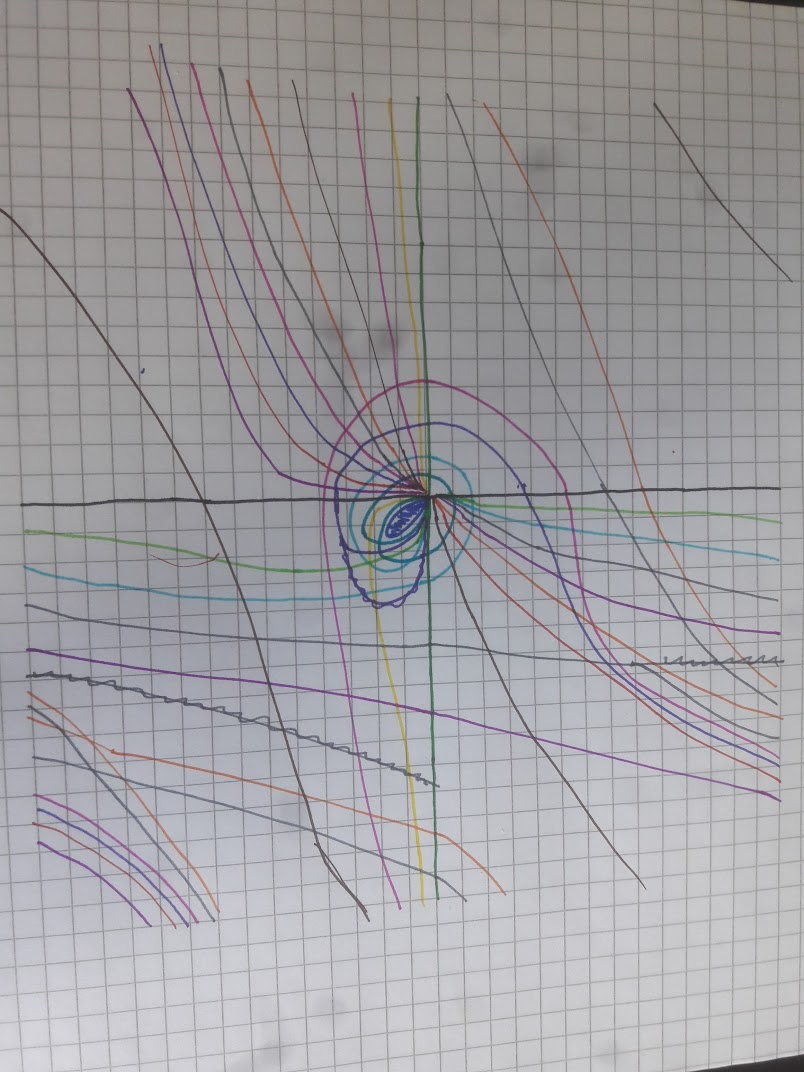
\includegraphics[scale=.42]{torus}}
	\caption{The universal cover of the $2$-triangulation of a torus with one hole and one marked point, represented in \cref{fig:torus}. It has five $2$-stars and all flips are sequential.}
	\label{fig:UCtorus}
\end{figure}

Triangulations are fundamental tools to understand and manipulate topological spaces.
Triangulations of surfaces are particularly interesting as they feature strong enumerative and structural combinatorial properties.
On the enumerative side, triangulated maps on surfaces are counted by surprising product formulas. % line of research started analytically by W.~Tutte in the sixties and actively developed by bijective approaches.
On the structural side, crossing-free collections of arcs between marked points on a given surface define a pure simplicial complex, whose facets are triangulations.
In particular, triangulations admit a natural flip operation that exchanges an arc~$\alpha$ with the other diagonal of the quadrangle formed by the two triangles containing~$\alpha$.
These structural properties were used for instance to provide a large and relevant family of examples of cluster algebras whose combinatorics is driven by the triangulations of a surface and the flips between them.

Triangulations can be interpreted as maximal crossing-free collections of arcs connecting a fixed collection of marked points on the surface.
An interesting line of research arises when considering maximal collections of arcs with ``few crossings''.
There are various relevant ways to restrict crossings.
One can require for instance that the arcs have at most $\ell$ crossings in total, or that there is no subset of $\ell+2$ mutually crossing arcs, or that each arc crosses at most $\ell$ other arcs, etc.
All these conditions translate natural restrictions forcing the intersection graph of the arcs to be a ``small graph''.
Namely, it corresponds to an intersection graph with at most $\ell$ edges, with no $(\ell+2)$-clique, or with maximal degree~$\ell$, etc.
Note that all these restrictions specialize to classical triangulations when~$\ell = 0$.
The first restriction (at most $\ell$ crossings) has been studied in details in~\cite{PilaudRue}.
In this note, we consider the second restriction (no subset of mutually crossing arcs)., which were already considered in the literature in the case of a disk.

A \defn{$k$-triangulation} of a convex $n$-gon is a maximal set of diagonals with no $(k+1)$-crossing, \ie no subset of $k+1$ mutually crossing diagonals.
They were introduced in~\cite{CapoyleasPach} and particularly studied in~\cite{Nakamigawa, DressKoolenMoulton, Jonsson1, Jonsson2, SerranoStump, PilaudSantos-multitriangulations}.
They feature some strong structural properties, which naturally generalize classical properties of the triangulations ($k=1$):
\begin{enumerate}[(i)]
\item All $k$-triangulations of the $n$-gon have $k(n-2k-1)$ edges~\cite{CapoyleasPach, Nakamigawa, DressKoolenMoulton}.
\item Any edge of length at least~$k + 1$ can be flipped and the graph of flips is regular and connected~\cite{Nakamigawa, DressKoolenMoulton}.
\item Any $k$-triangulation decomposes into a complex of $k$-stars~\cite{PilaudSantos-multitriangulations}.
\item The set of $k$-triangulations of the $n$-gon is enumerated by a determinant of Catalan numbers~\cite{Jonsson1, Jonsson2}. It is thus in bijection with families of $k$ mutually non-crossing Dyck paths~\cite{SerranoStump}.
\end{enumerate}

The objective of this note is to introduce the good notion of $k$-triangulations on a surface such that properties (i) to (iii) above hold.
For this, we start from a surface~$\surface$ with boundaries and fix some marked points on its boundaries.
We then consider collections of arcs (up to homotopy) joining marked points with no $(k+1)$-crossing.
The right notion of $(k+1)$-crossings requires to consider the universal cover~$\bar\surface$ of the surface~$\surface$.
Namely, a $(k+1)$-crossing in~$\surface$ is the projection of a set of $k+1$ mutually crossing arcs in the universal cover~$\bar\surface$.
The subtlety here is that there are collections of pairwise crossing arcs of~$\surface$ which do not admit pairwise crossing representatives on the universal cover~$\bar\surface$.
Armed with this solid notion of $k$-triangulations on~$\surface$, we are able to prove analogues of properties (i) and (iii) above, and to discuss property (ii).

In fact, our approach is to first consider $k$-triangulations on a disk with infinitely many vertices (see \cref{sec:infiniteMultitriangulations}).
Under rather weak assumptions that ensure a sort of local finiteness, we show that these infinite $k$-triangulations decompose into $k$-stars and admit a flip operation.
We then consider $k$-triangulations on surfaces as quotients of periodic infinite $k$-triangulations by Fuchsian groups (see \cref{sec:multitriangulationsSurfaces}).
Most structural properties of infinite triangulations are preserved by this quotient.
As discussed at the end of this note, the main difficulty remains in the behavior of the periodicity under the flip operation.

%%%%%%%%%%%%%%%%%%%%%%%%%%%%%%%%%%%%%%

\section{Multitriangulations of infinite polygons}
\label{sec:infiniteMultitriangulations}

The objective of this section is to study $k$-triangulations of an infinite polygon.
The key property here is the existence of the $k$-star decomposition established for $k$-triangulations of a convex $n$-gon in~\cite{PilaudSantos-multitriangulations}.
In fact, many arguments of~\cite{PilaudSantos-multitriangulations} easily adapt to the case of an infinite polygon assuming some sort of local finiteness properties that we present first.

%%%%%%%%%%%%

\subsection{Infinite polygons}

We now provide a proper definition of infinite polygon (\cref{def:infinitePolygon}) and of two local finiteness conditions (\cref{def:tidyPolygon,def:EV-finite}) that will be relevant later.

\begin{definition}
\label{def:infinitePolygon}
A \defn{polygon}~$P$ is a cyclically ordered set, that might be finite or infinite.
We write~$a \cl b \cl c$ for the cyclic order.
The elements of~$P$ are called \defn{points} and pairs of elements of~$P$ are called \defn{diagonals}.
For two points~$a,b \in P$, let~$[a,b] \eqdef \set{c \in P}{a \le c \le b}$, and define similarly the intervals~$[a,b[$, $]a,b]$ and~$]a,b[$ (with open brackets for strict inequalitites).
Two diagonals~$(a,c)$ and~$(b,d)$ of~$P$ \defn{cross} if~$a \cl b \cl c \cl d$.
\end{definition}

\begin{definition}
\label{def:tidyPolygon}
If $x$ and $y$ are two points of a polygon~$P$ such that the interval~$]x,y[$ is empty, we say that~$x$ is the \defn{predecessor} of~$y$ and that~$y$ is the \defn{successor} of~$x$, and we use the notations~$y = x+1$ and~$x = y-1$. A polygon~$P$ is \defn{tidy} if each point of~$P$ has both a predecessor and a successor. In particular, finite polygons are tidy.
\end{definition}

\begin{definition}
\label{def:EV-finite}
A set~$X$ of diagonals of a polygon~$P$ is 
\begin{itemize}
\item \defn{\ef} if each diagonal of~$X$ is crossed by a finite number of diagonals of~$X$,
\item \defn{\vf} if each vertex of~$P$ is incident to finitely many diagonals of~$X$.
\end{itemize}
\end{definition}

%%%%%%%%%%%%

\subsection{Infinite multitriangulations}

We now define $k$-triangulations of infinite polygons exactly as those of finite convex polygons.

\begin{definition}
A \defn{$k$-crossing} of a polygon~$P$ is a set of~$k$ pairwise crossing diagonals of~$P$.
A \defn{$k$-triangulation} of~$P$ is an inclusion-maximal set of diagonals of~$P$ with no $(k+1)$-crossing.
\end{definition}

\begin{definition}
The \defn{length} of a diagonal~$(a,b)$ of a polygon~$P$ is the minimum~$\ell(a,b)$ of~$|{]a,b[}|$ and~$|{]b,a[}|$ (note that this might be infinite).
A diagonal~$(a,b)$ with~$\ell(a,b) > k$ (resp.~$\ell(a,b) = k$, resp.~$\ell(a,b) < k$) is a \defn{$k$-relevant} (resp.~\defn{$k$-boundary}, resp.~\defn{$k$-irrelevant}) diagonal.
\end{definition}

\begin{remark}
\label{rem:kboundary}
Observe that a diagonal contained in a $(k+1)$-crossing must be $k$-relevant.
Therefore, any \ktg contains all $k$-irrelevant and $k$-boundary diagonals by maximality.
\end{remark}

As observed in~\cite{PilaudSantos-multitriangulations}, many combinatorial properties of $k$-triangulations are better understood from their decompositions into $k$-stars, which generalize triangles in triangulations.

\begin{definition}
A \defn{$k$-star} of a polygon~$P$ is a set of diagonals of~$P$ of the form~$\set{(s_i, s_{i+k})}{0 \le i \le 2k}$ where~$s_0 \cl \dots \cl s_{2k}$ (where the indices are understood modulo~$2k+1$).
\end{definition}

\begin{definition}
An \defn{angle} of a set~$X$ of diagonals of a polygon~$P$ is a pair of diagonals~$\{(u,v), (v,w)\}$ with~$u \cl v \cl w$ such that~$X$ contains no diagonal of the form~$(v,t)$ with~$w \cl t \cl u$. The angle is denoted by~$\angle(u,v,w)$ and we say that~$v$ is the \defn{apex} of~$\angle(u,v,w)$. An angle is \defn{$k$-relevant} if its two diagonals are $k$-relevant or $k$-boundary edges. %A set~$Y$ of diagonals of~$P$ crosses the angle~$\angle(u,v,w)$ if each diagonal of~$Y$ crosses both~$(u,v)$ and~$(v,w)$. 
\end{definition}

One of the objectives of this paper is to prove the following structural results on infinite $k$-triangulations.

\begin{theorem}
\label{thm:structureInfinite}
Let~$T$ be a \ef \ktg of a tidy polygon~$P$. Then:
\begin{enumerate}
\item Each $k$-relevant angle of~$T$ is contained in precisely one $k$-star of~$T$.
\item Each $k$-relevant (resp.~$k$-boundary, resp.~$k$-irrelevant) diagonal of~$T$ is contained in precisely two (resp.~one, resp.~no) $k$-stars of~$T$.
\item For any $k$-relevant diagonal~$e$ of~$T$, there exists a unique diagonal~$f$ not in~$T$ such that~$T \symdif \{e,f\}$ is another $k$-triangulation. The diagonal~$f$ only depend on the two $k$-stars of~$T$ containing~$e$.
\item Let~$P'$ denote a polygon obtained by replacing $k+1$ consecutive points of~$P$ by~$k$ points. Then there exists a flattening (resp.~inflating) operation that transforms the \ktg{}s of~$P$ into the \ktg{}s of~$P'$ (resp.~and \viceversa).
%\item For any point~$p$ of the plane, the $k$-depth of~$p$ in~$P$ is equal to the sum of the winding numbers around~$p$ of the $k$-stars of~$T$.
\end{enumerate}
\end{theorem}

%We prove \cref{thm:structureInfinite} in \cref{subsec:prfInfinite}.
%
%\begin{remark}
%\begin{itemize}
%\item flip graph connected? Increasing flip graph?
%\item duality with pseudoline arrangements?
%\item $k$-arboresence? connection to $k$-edge-connected but not locally $(k+1)$-edge-connected.
%\end{itemize}
%\end{remark}

%%%%%%%%%%%%

%\subsection{Some counter-examples}
%
%\begin{ce}
%The polygon of a periodic \ktg is not necessarily a \nbd.
%\end{ce}
%\begin{proof}
%
%\end{proof}
%
%\begin{ce}
%A periodic \ef \ktg may have angles that are not crossed by a $(k-1)$-crossing.
%\end{ce}
%\begin{proof}
%
%\end{proof}
%
%\begin{ce} 
%A periodic \ktg may not be \ef.
%\end{ce}
%\begin{proof}
%
%\end{proof}
%
%\begin{ce}
%A \ef \ktg of a \nbd is not necessarily \vf.
%\end{ce}
%\begin{proof}
%k=1
%\end{proof}

%%%%%%%%%%%%

\subsection{Proof of \cref{thm:structureInfinite}}
\label{subsec:prfInfinite}

The end of this section is devoted to the proof of \cref{thm:structureInfinite}.
We follow the ideas of the proof of~\cite{PilaudSantos-multitriangulations} in the case of finite convex polygons, but we adapt the arguments to show that the conditions of $E$-finiteness and tidiness suffice to obtain the same result in the case of infinite polygons.

%%%

\subsubsection{$(k-1)$-crossings crossing an angle}

We first study the $(k-1)$-crossings that cross a given angle in a $k$-triangulation.

\begin{definition}
A $(k-1)$-crossing~$A = \{a_1, \dots, a_{k-1}\}$ \defn{crosses} an angle~$\angle(u,v,w)$ if each diagonal~$a_i$ crosses both diagonals~$(u,v)$ and~$(v,w)$.
\end{definition}

We stick to the convention to label the diagonals of~$A$ by~$a_i \eqdef (a^\bullet_i, a^\circ_i)$ in such a way that $u \cl a^\bullet_1 \cl \dots \cl a^\bullet_{k-1} \cl v \cl a^\circ_1 \cl \dots \cl a^\circ_{k-1} \cl w$. We use this convention throughout this section without further notice.

\begin{lemma}
\label{lem:tidyExists}
In a \ktg $T$ of a tidy polygon, any $k$-relevant angle is crossed by a $(k-1)$-crossing.
\end{lemma}

\begin{proof}
Any angle~$\angle(u,v,w)$ is crossed by the $(k-1)$-crossing~$\set{(v-k+i, v+i)}{i \in [k-1]}$ of $k$-boundary diagonals, which belongs to the \ktg $T$ by \cref{rem:kboundary}.
\end{proof}

\begin{definition}
Let $\angle(u,v,w)$ be a $k$-relevant angle of $T$.
For two diagonals~$a$ and~$b$ of $T$ that cross $\angle(u,v,w)$, we say that $a$ is \defn{$v$-farther} than $b$ if $u \cl a^\bullet \cle b^\bullet \cl v \cl b^\circ \cle a^\circ \cl w$. For two $(k-1)$-crossings $A = \{a_1, \dots, a_{k-1}\}$ and $B = \{b_1, \dots, b_{k-1}\}$ that cross $\angle(u,v,w)$, we say that $A$ is \defn{$v$-farther} than $B$ if $a_i$ is $v$-farther than $b_i$ for every $i \in [k-1]$. We say that $A$ is the \defn{$v$-farthest} $(k-1)$-crossing if it is $v$-farther than any other $(k-1)$-crossing that crosses~$\angle(u,v,w)$.
\end{definition}

\begin{lemma}
In a \ktg, the set of $(k-1)$-crossings crossing a given $k$-relevant angle forms a distributive lattice.
\end{lemma}

\begin{proof}
Consider two $(k-1)$-crossings $A = \{a_1, \dots, a_{k-1}\}$ and $B = \{b_1, \dots, b_{k-1}\}$ that cross the angle~$(u,v,w)$.

There is no $i$ such that $a_i$ crosses $b_i$. 
Indeed, suppose $a^\bullet_i \cl b^\bullet_i \cl v \cl a^\circ_i \cl b^\circ_i$. Then $\{(u, v), a_1, \dots, a_i, b_i, \dots, b_{k-1}\}$ forms a $(k+1)$-crossing. 
Similarly, if $b^\bullet_i \cl a^\bullet_i \cl v \cl b^\circ_i \cl a^\circ_i$, then $\{(u, v), b_1, \dots, b_i, a_i, \dots, a_{k-1}\}$ forms a $(k+1)$-crossings.
Hence $A$ and $B$ are edgewise comparable.

We define the meet (resp.~join) of $A$ and $B$ as their edgewise minimum (resp.~maximum). With this definition it is easy to see that we obtain a distributive lattice.
\end{proof}

\begin{lemma}
\label{lem:efMax}
In a \ef \ktg, for any angle~$\angle(u,v,w)$ crossed by at least one $(k-1)$-crossing, there exists a $v$-farthest $(k-1)$-crossing that crosses~$\angle(u,v,w)$.
\end{lemma}

\begin{proof}
By \ef{}ness, the angle~$\angle(u,v,w)$ is crossed by a finite number of $(k-1)$-crossings. Hence the distributive lattice of such $(k-1)$-crossings is finite, and has a unique maximum.
\end{proof}

Combining \cref{lem:tidyExists,lem:efMax}, we obtain the following statement.

\begin{corollary}
\label{coro:farthestTidy}
In a \ef \ktg of a tidy polygon, for any angle~$\angle(u,v,w)$, there exists a $v$-farthest $(k-1)$-crossing that crosses~$\angle(u,v,w)$.
\end{corollary}

%%%

\subsubsection{Any $k$-relevant angle belongs to a $k$-star}

We now use the existence of a $v$-farthest $(k-1)$-crossing to show that the angle~$\angle(u,v,w)$ belongs to a $k$-star.

\begin{proposition}
\label{prop:angleBelongStar}
For any angle~$\angle(u,v,w)$ of a \ktg, if there is a $v$-farthest $(k-1)$-crossing that crosses~$\angle(u,v,w)$, then~$\angle(u,v,w)$ belongs to a $k$-star.
\end{proposition}

\begin{proof}
The proof follows the same lines as that of~\cite[Thm.~4.1]{PilaudSantos-multitriangulations}. We repeat the argument here for the convenience of the reader.

Let $E=\{e_1, \dots , e_{k-1}\}$ be the $v$-farthest $(k-1)$-crossing that crosses $\angle(u, v, w)$.
We will prove that the diagonals $(u, e^\circ_1), (e^\bullet_1, e^\circ_2) \dots (e^\bullet_{k-2}, e^\circ_{k-1}), (e^\bullet_{k-1}, w)$ are in $T$ such that the points $u$, $e^\bullet_1, \dots, e^\bullet_{k-1}$, $v$, $e^\circ_1, \dots, e^\circ_{k-1}$, $w$ are the vertices of a $k$-star of $T$ containing the angle $\angle(u, v, w)$. 

To get this result, we use two steps, illustrated in \cref{fig:exProofStar}: first we prove that $\angle(e^\bullet_1, e^\circ_1, u)$ is an angle of $T$, and then we prove that the diagonals $e_2, \dots, e_{k-1}, (v, w)$ form a $(k-1)$-crossing intersecting $\angle(e^\bullet_1, e^\circ_1, u)$ and $e^\circ_1$-farthest (so that we can reiterate the argument).


\begin{figure}
  \centering
  \begin{subfigure}[b]{.48\textwidth}
	\centering
	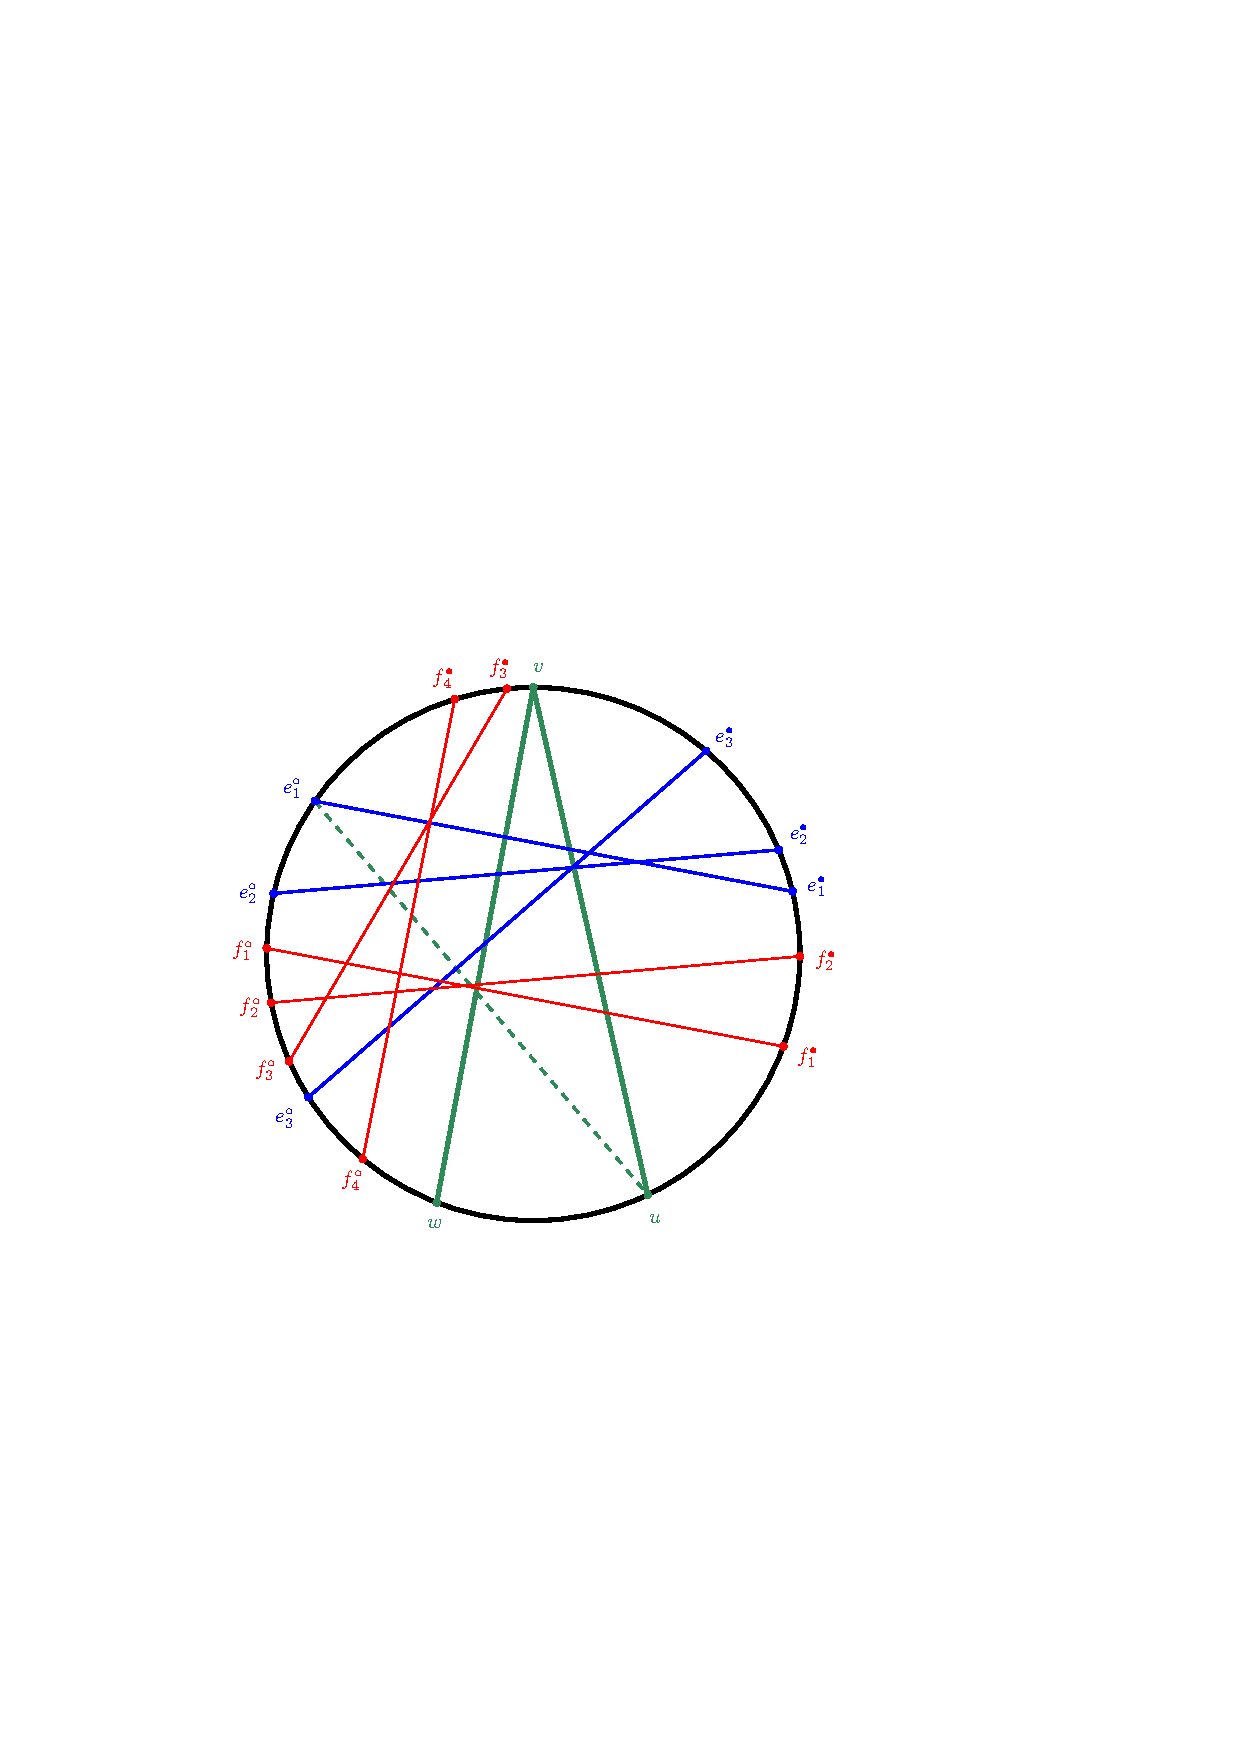
\includegraphics[width=\textwidth,page=1]{exProofStar}
  \end{subfigure}
  \begin{subfigure}[b]{.48\textwidth}
    \centering
    \includegraphics[width=\textwidth,page=2]{exProofStar}
  \end{subfigure}
  \caption{Illustrations of the first and second steps of the proof of \cref{prop:angleBelongStar}. In both case, $k=4$, and on the left, $\ell=2$.}
  \label{fig:exProofStar}
\end{figure}

\medskip
\paragraph{\bf First step.}
Suppose that $(u, e^\circ_1)$ is not in $T$. 
Since $T$ is a $k$-triangulation, there is a $k$-crossing $F=\{f_1, \dots, f_k\}$ (with $u \cl f^\bullet_1 \cl \cdots \cl f_k \cl e'_1 \cl f'_1 \cl \cdots \cl f'_k \cl u$) that prevents the diagonal~$(u, e^\circ_1)$. We will now exhibit a $(k-1)$-crossing of the form~$\{f_1, \dots, f_\ell, e_{\ell+1}, \dots, e_{k-1}\}$ that will cross~$\angle(u,v,w)$ and be $v$-farther than~$E$, contradicting the maximality of~$E$.

Note first that~$f^\bullet_k \in [v, e^\circ_1[$, as otherwise~$F \cup \{(u, v)\}$ would form a $(k + 1)$-crossing.
Additionnaly, $f^\circ_k \in {]e^\circ_1, w]}$, as otherwise $E \cup \{(v,w), (f^\bullet_k, f^\circ_k)\}$ would form a $(k + 1)$-crossing. 
Consequently, we have~$f^\circ_1 \in {]e^\circ_1, w[}$ $e^\circ_1 \cl f^\circ_1 \cl \cdots \cl f^\circ_{k-1} \cl w$.

Let $\ell = \max \set{j\in[k-1]}{\, f^\circ_i \in {]e^\circ_i, w[} \text{ for all } i \le j}$.
Then $f^\bullet_i \in {]u, e^\bullet_i]}$ for any $i \le \ell$, as otherwise $\{e_1, \dots , e_i, f_i, \dots , f_k\}$ would form a $(k + 1)$-crossing.
Thus~$f_i$ crosses~$\angle(u,v,w)$ and is $v$-farther than~$e_i$ for any~$i \le \ell$.
Furthermore, we have $f^\circ_\ell \cl f^\circ_{\ell+1} \cl e^\circ_{\ell+1}$ (by maximality of~$\ell$) and~$f^\bullet_\ell \cl e^\bullet_{\ell} \cl e^\bullet_{\ell+1}$, so that~$f_\ell$ crosses~
$e_{\ell+1}$. 
Consequently, we get a $(k-1)$-crossing $\{f_1, \dots , f_\ell, e_{\ell+1}, \dots , e_{k-1}\}$ which is $v$-farther than $\{e_1, \dots , e_{k-1}\}$, contradicting the maximality of~$E$. 
We conclude that~$(u, e^\circ_1)$ belongs to~$T$.

Suppose now that~$\angle(e^\bullet_1, e^\circ_1, u)$ is not an angle of~$T$. 
Then there exists $e^\bullet_0 \in {]u, e^\bullet_1[}$ such that $(e^\bullet_0, e^\circ_1) \in T$. 
But then the $(k-1)$-crossing $\{(e^\bullet_0, e^\circ_1), e_2, \dots, e_{k-1}\}$ is $v$-farther than~$E$. 
This implies that~$\angle(e^\bullet_1, e^\circ_1, u)$ is an angle of~$T$.

\medskip
\paragraph{\bf Second step.}
Assume now that there exists a $(k-1)$-crossing~$F=\{f_2, \dots , f_k\}$ that crosses $\angle(e^\bullet_1, e^\circ_1, u)$ and is $e^\circ_1$-farther than the $(k-1)$-crossing $\{e_2, \dots, e_{k-1}, (v, w)\}$.

Note first that~$f_k = (v,w)$. Indeed, since~$f_k$ is $e^\circ_1$-farther than~$(v,w)$, we have~$f^\bullet_k \in {]e^\bullet_1, v]}$ and~$f^\circ_k \in [w,u[$. Therefore~$f^\bullet_k = v$ (as otherwise~$\{(u,v), e_1\} \cup F$ would form a $(k+1)$-crossing), and~$f^\circ_k = w$ (since~$\angle(u,v,w)$ is an angle of~$T$).

Since~$f_k = (v,w)$, we obtain that~$\{e_1, f_2, \dots, f_{k-1}\}$ is a $(k-1)$-crossing that crosses~$\angle(u,v,w)$. For any $i \in [2,k-1]$, the diagonal~$f_i$ is $e^\circ_1$-farther than~$e_i$, and thus also $v$-farther than~$e_i$. Therefore, $\{e_1, f_2, \dots, f_{k-1}\}$ is $v$-farther than~$E$, contradicting the maximality of~$E$.
\end{proof}

Combining \cref{coro:farthestTidy} and \cref{prop:angleBelongStar}, we obtain the proof of \cref{thm:structureInfinite}\,(1).

\begin{corollary}
\label{coro:angleInStar}
In a \ef \ktg of a tidy polygon, any $k$-relevant angle belongs to a $k$-star.
\end{corollary}

%%%

\subsubsection{Any $k$-relevant diagonal belongs to two $k$-stars}

We now use $k$-relevant angles to show that any $k$-relevant (resp.~$k$-boundary, resp.~$k$-irrelevant) diagonal of a $k$-triangulation~$T$ is contained in precisely two (resp.~one, resp.~no) $k$-stars of~$T$.

\begin{lemma}
When $k\geq 2$, any \ef \ktg of a tidy polygon is also \vf.
\end{lemma}

\begin{proof}
Any $k$-boundary diagonal~$e$ surrounding a given vertex~$v$ intersects all diagonals adjacent to~$v$.
As the $k$-triangulation is \ef, the diagonal~$e$ intersects finitely many diagonals, thus~$v$ has finite degree.
Note that the reverse implication is wrong: there are \vf $k$-triangulations that are not \ef.
\end{proof}

\begin{lemma}
\label{lem:diagsInAngles}
Any $k$-relevant (resp.~$k$-boundary) diagonal of a \vf \ktg belongs to four (resp.~two) $k$-relevant angles.
\end{lemma}

\begin{proof}
Consider a $k$-relevant diagonal~$e$ in a \vf \ktg $T$.
By \vf{}ness, both endpoints of~$e$ have finite degree.
Then the diagonals just before and just after~$e$ around the endpoints of~$e$ are all either $k$-relevant or $k$-boundary diagonals and thus define four $k$-relevant angles containing~$e$.
The proof is similar for a $k$-boundary diagonal, except only two of the incident angles are $k$-relevant
\end{proof}

Combining \cref{lem:diagsInAngles,coro:angleInStar}, we obtain the proof of \cref{thm:structureInfinite}\,(2).

\begin{corollary}
Any $k$-relevant (resp.~$k$-boundary, resp.~$k$-irrelevant) diagonal of a \ef $k$-triangulation~$T$ of a tidy polygon is contained in precisely two (resp.~one, resp.~no) $k$-stars of~$T$.
\end{corollary}

\begin{proof}
Any $k$-relevant diagonal~$e$ is contained in four $k$-relevant angles by \cref{lem:diagsInAngles}, each contained in a $k$-star of~$T$ by \cref{coro:angleInStar}.
As the two angles on the same side of~$e$ belong to the same $k$-star of~$T$, we obtain precisely two $k$-stars of~$T$ containing~$e$.
The proof is similar for a $k$-boundary diagonal, except that only one side gives rise to a $k$-star of~$T$.
\end{proof}

%%%

\subsubsection{Mutual position of two $k$-stars}



%%%

\subsubsection{Flipping a $k$-relevant diagonal}

cf Pilaud Santos. to be adapted to the infinite case, but shouldn't need any additional hypothesis. quite long though : section 3.

%%%

\subsubsection{Flattening a boundary $k$-star, inflating a boundary $k$-crossing}

\begin{figure}
  \centering
  \begin{subfigure}[b]{.48\textwidth}
	\centering
	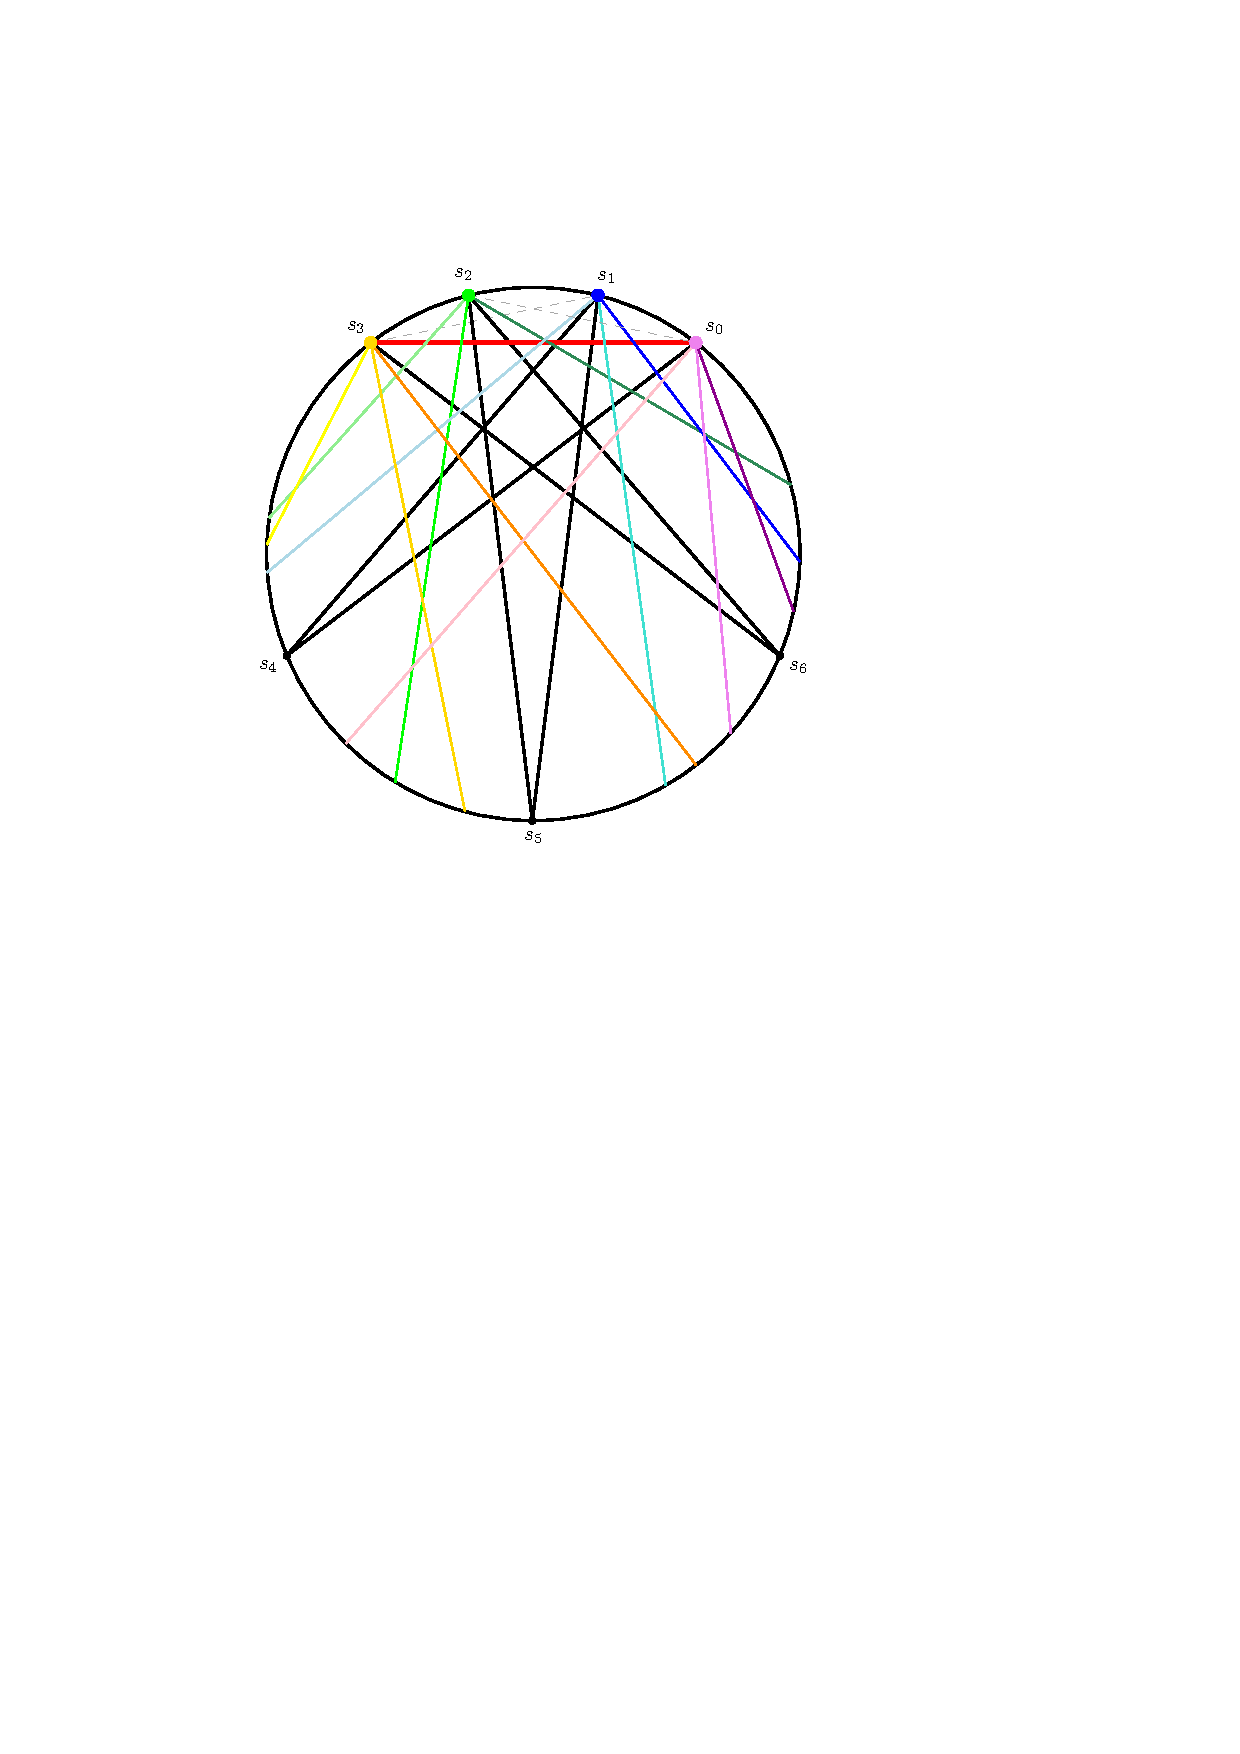
\includegraphics[width=\textwidth,page=1]{exFlattening}
  \end{subfigure}
  \begin{subfigure}[b]{.48\textwidth}
    \centering
    \includegraphics[width=\textwidth,page=2]{exFlattening}
  \end{subfigure}
  \caption{Illustrations of the flattening of a boundary $k$-star, with $k=3$.}
  \label{fig:exProofStar}
\end{figure}

%%%%%%%%%%%%%%%%%%%%%%%%%%%%%%%%%%%%%%

\section{Multitriangulations of a general surface}
\label{sec:multitriangulationsSurfaces}
 
%%%%%%%%%%%%

\subsection{Surfaces, universal cover, $(k+1)$-crossings and $k$-triangulations}

\begin{definition}
Consider a connected surface~$\surface$ with boundary and a set~$V$ of marked points on the boundary. An \defn{arc} of~$\surface$ is a curve on~$\surface$ connecting two points of~$V$ and whose interior is disjoint from the boundary of~$\surface$. We consider arcs up to homotopy relative to their endpoints in~$\surface$ and we disallow arcs homotopic to a boundary segment of~$\surface$.
\end{definition}

%\begin{remark}
%We could also consider the case of a surface with no marked points on some boundaries. Be careful that the definition of $k$-relevant, $k$-boundary and $k$-irrelevant diagonals are not clear anymore in that case.
%\end{remark}

In this section, we will use the representation of surfaces as quotients of the hyperbolic plane by Fuchsian groups.
As we only use the combinatorial aspects of this description, we take the liberty to remain quite informal on this representation.
Any surface~$\surface$ can be constructed from a polygon~$P$ by glueing some of its edges (the unglued edges of the polygon form the boundary of the surface~$\surface$).
When the surface has genus~$g > 1$ and no boundary, there is a subgroup~$\Gamma$ of isometries of the hyperbolic disk~$\disk$ so that this polygon~$P$ is the fundamental domain of~$\Gamma$, the surface~$\surface$ is isomorphic to the quotient~$\disk/\Gamma$, and the disk~$\disk$ is the universal cover of the surface~$\surface$.
When the surface has boundaries, we use a similar representation.
We embed $P$ in the hyperbolic disk~$\disk$ and we consider the subgroup~$\Gamma$ of isometries of the hyperbolic disk~$\disk$ generated by the identifications of the edges of~$P$ dictated by the surface~$\surface$.
The universal cover of the surface~$\surface$ is then the part~$\bar\surface$ of the hyperbolic disk~$\disk$ tiled by all images of~$P$ by~$\Gamma$.
This representation is illustrated for instance in \cref{fig:UCtorus}.

\begin{definition}
A \defn{$k$-crossing} on~$\surface$ is a collection~$\alpha_1, \dots, \alpha_k$ (possibly with repetition) of $k$ arcs of~$\surface$ which admit pairwise crossing representatives~$\bar\alpha_1, \dots, \bar\alpha_k$ in the universal cover~$\bar\surface$.
A \defn{$k$-triangulation} of~$P$ is an inclusion maximal set of diagonals of~$P$ with no $(k+1)$-crossing.
\end{definition}

\begin{remark}
Be careful: a $k$-crossing on~$\surface$ is NOT a collection of pairwise crossing arcs of~$\surface$. Namely, there are collections of pairwise crossing arcs of~$\surface$ which do not admit pairwise crossing representatives. The simplest examples are self-crossing arcs, whose representation may not be self-crossing. Further examples are given in \cref{fig:notkcrossing}.
\vincent{Todo.}
\end{remark}

\begin{example}

\end{example}


%%%%%%%%%%%%

\subsection{Structural properties}

\begin{figure}[t]
	\capstart
	\centerline{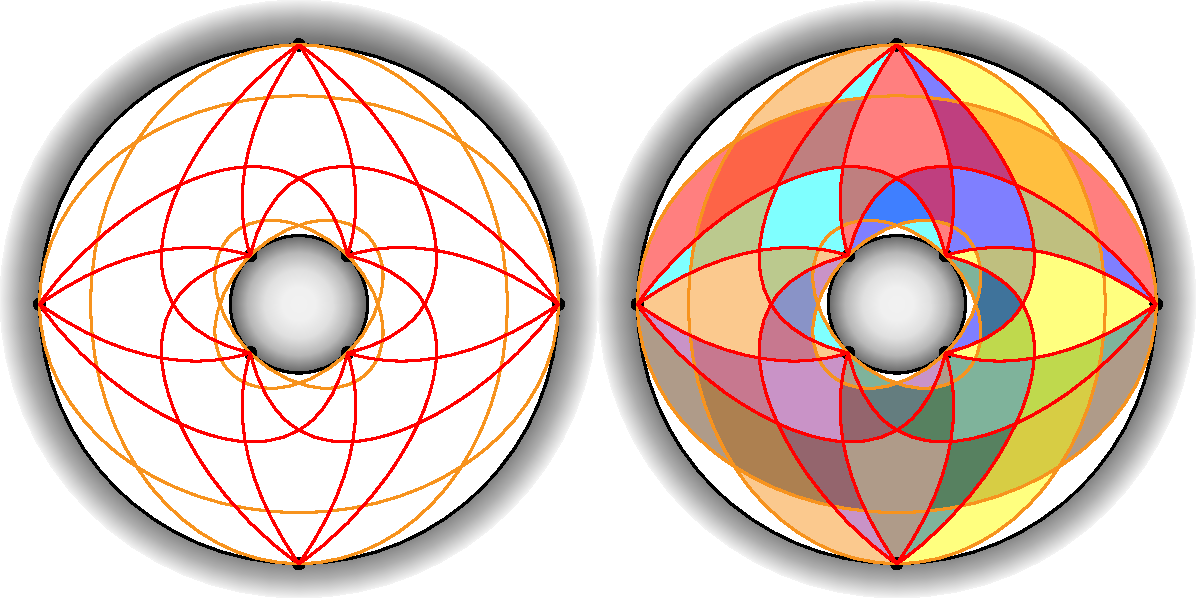
\includegraphics[scale=.5]{2triangCylinderStars}}
	\caption{A $2$-triangulation of a cylinder, where $2$-relevant edges are red while $2$-boundary edges are orange (left) and its decomposition into $2$-stars (right).}
	\label{fig:starsSurface}
\end{figure}

\begin{theorem}
\label{thm:structureSurface}
Any \ktg of a surface of genus~$g$ with~$b$ boundaries and~$n$ marked points has precisely $n + 2k(2g + b - 2)$ $k$-stars and $kn + k(2k + 1)(2g + b - 2)$ $k$-relevant arcs.
\end{theorem}

\begin{proof}
There are various possible proofs of this statement, none of them is really clean at the moment.

The first (original) proof is based on cutting along edges.
Start from a $k$-triangulation~$T$ of a surface~$\surface$ with at least~$2k+1$ marked points, genus~$g$ and $b$ boundaries.
If~$T$ has no $k$-relevant edge, then~$T$ is the complete graph on $2k+1$ vertices, has a single $k$-star, and $\surface$ is a disk.
Otherwise, pick an arbitrary $k$-relevant edge~$e$ of~$T$.
Cut along~$e$, create $k-1$ new marked points on each side of~$e$, and rearrange the branches of the stars that cross~$e$ to these new marked points (there is a unique way to do this rearrangement).
This operation, illustrated in \cref{fig:cutSurface}, is easier to see on the disk, and can then be extended to surfaces using the universal cover.
%
\begin{figure}[t]
	\capstart
	\centerline{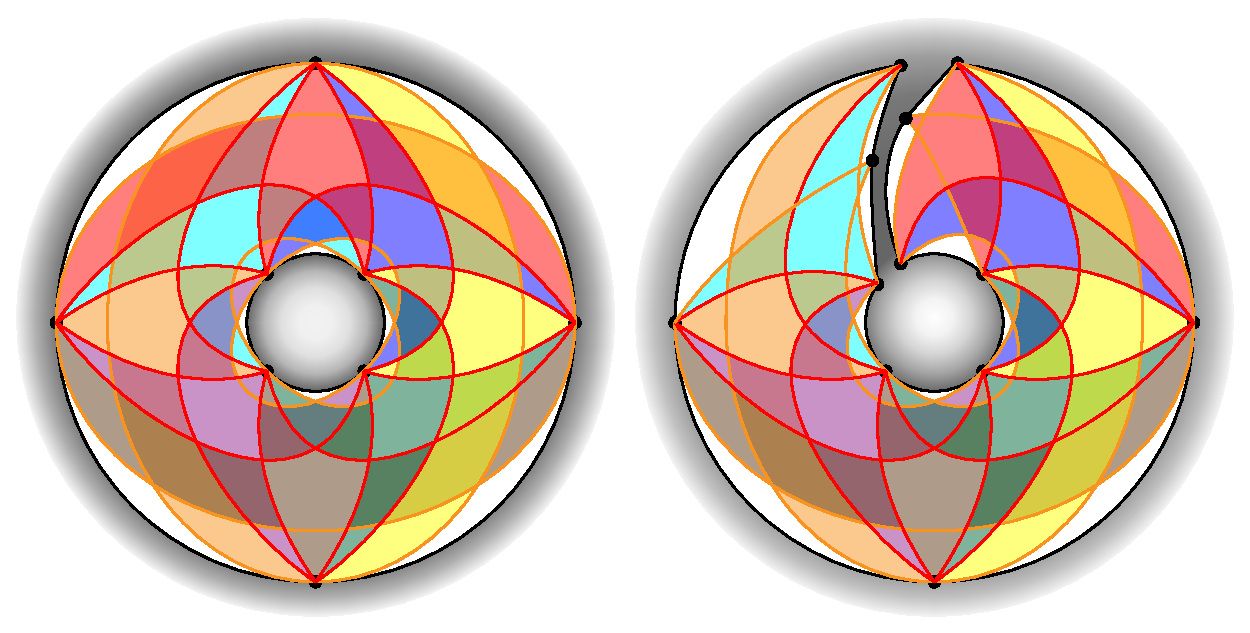
\includegraphics[scale=.5]{2triangCylinderCut}}
	\caption{Cutting a $2$-triangulation of a cylinder along a $2$-relevant edge.}
	\label{fig:cutSurface}
\end{figure}
%
We obtain a new $k$-triangulation~$T'$ on a new surface~$\surface'$ (not necessarily connected).
Note that
\begin{enumerate}
\item the $k$-triangulations~$T$ and~$T'$ have the same number of $k$-stars,
\item the surface~$\surface'$ has $n' = n+2k$ marked points (as we have duplicated the endpoints of~$e$ and we have created $2k-2$ new marked points),
\item the genius~$g'$ and number of boundaries~$b'$ of the surface~$\surface'$ depend on the choice of~$e$:
	\begin{itemize}
	\item if the endpoints of~$e$ belong to the same connected component of~$\surface$, then we cut a handle and thus~$g' = g-1$ and $b' = b+1$,
	\item if the endpoints of~$e$ belong to distinct connected components of~$\surface$, then we cut a border and thus~$g' = g$ and~$b' = b-1$.
	\end{itemize}
	But in both cases, $2g'+b' = 2g+b-1$.
\end{enumerate}
We conclude that $T'$ has indeed $n + 2k(2g + b -2) = n' + 2k(2g' + b - 2)$ $k$-stars.

\medskip
I am working on another proof, but I can't yet make it work correctly.

\medskip
Once we know the number of $k$-stars, the number of $k$-relevant edges immediately follows by double counting.
Indeed, since
\begin{itemize}
\item each $k$-relevant edge belongs to two $k$-stars while each $k$-boundary edge belongs to one $k$-star,
\item each $k$-star contains $2k+1$ edges which are all either $k$-relevant of $k$-boundary,
\item there are precisely $n$ $k$-boundary edges,
\end{itemize}
we obtain that the number $s$ of $k$-stars and the number $r$ of $k$-relevant edges in a $k$-triangulation are related by
\(
2r + n = (2k+1) s
\)
from which we derive that
\[
r = \big( (2k+1)s-n \big)/2 = kn + k(2k + 1)(2g + b - 2).
\qedhere
\]
\end{proof}

\begin{figure}[t]
	\capstart
	\centerline{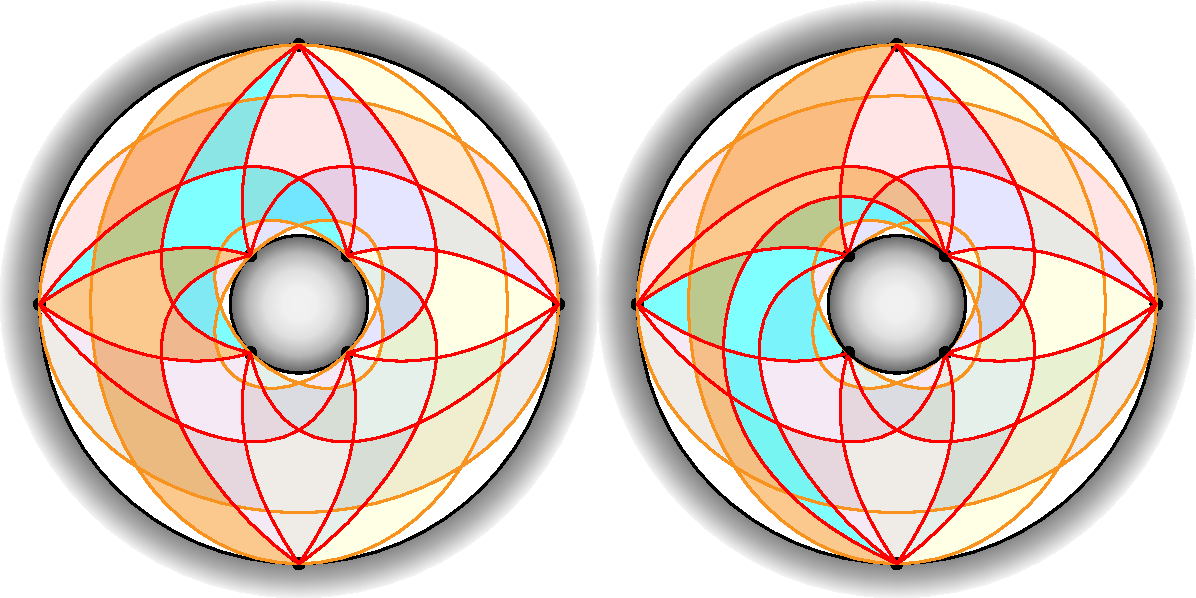
\includegraphics[scale=.5]{2triangCylinderFlip}}
	\caption{A flip of a $2$-relevant edge in a $2$-triangulation of a cylinder.}
	\label{fig:flipSurface}
\end{figure}


\begin{remark}
\begin{itemize}
\item \cite[Lem.~7.10]{PilaudSantos-multitriangulations}: Any $k$-triangulation of the $n$-gon contains at most $k(n-2p-1)$ $p$-relevant diagonals. Extension for surfaces.
\item flip graph connected? Increasing flip graph? Is it a lattice? (use bracket vectors)
\item duality? Line space of the surface?
\item punctures?
\end{itemize}
\end{remark}


\begin{figure}[h]
	\capstart
	\centerline{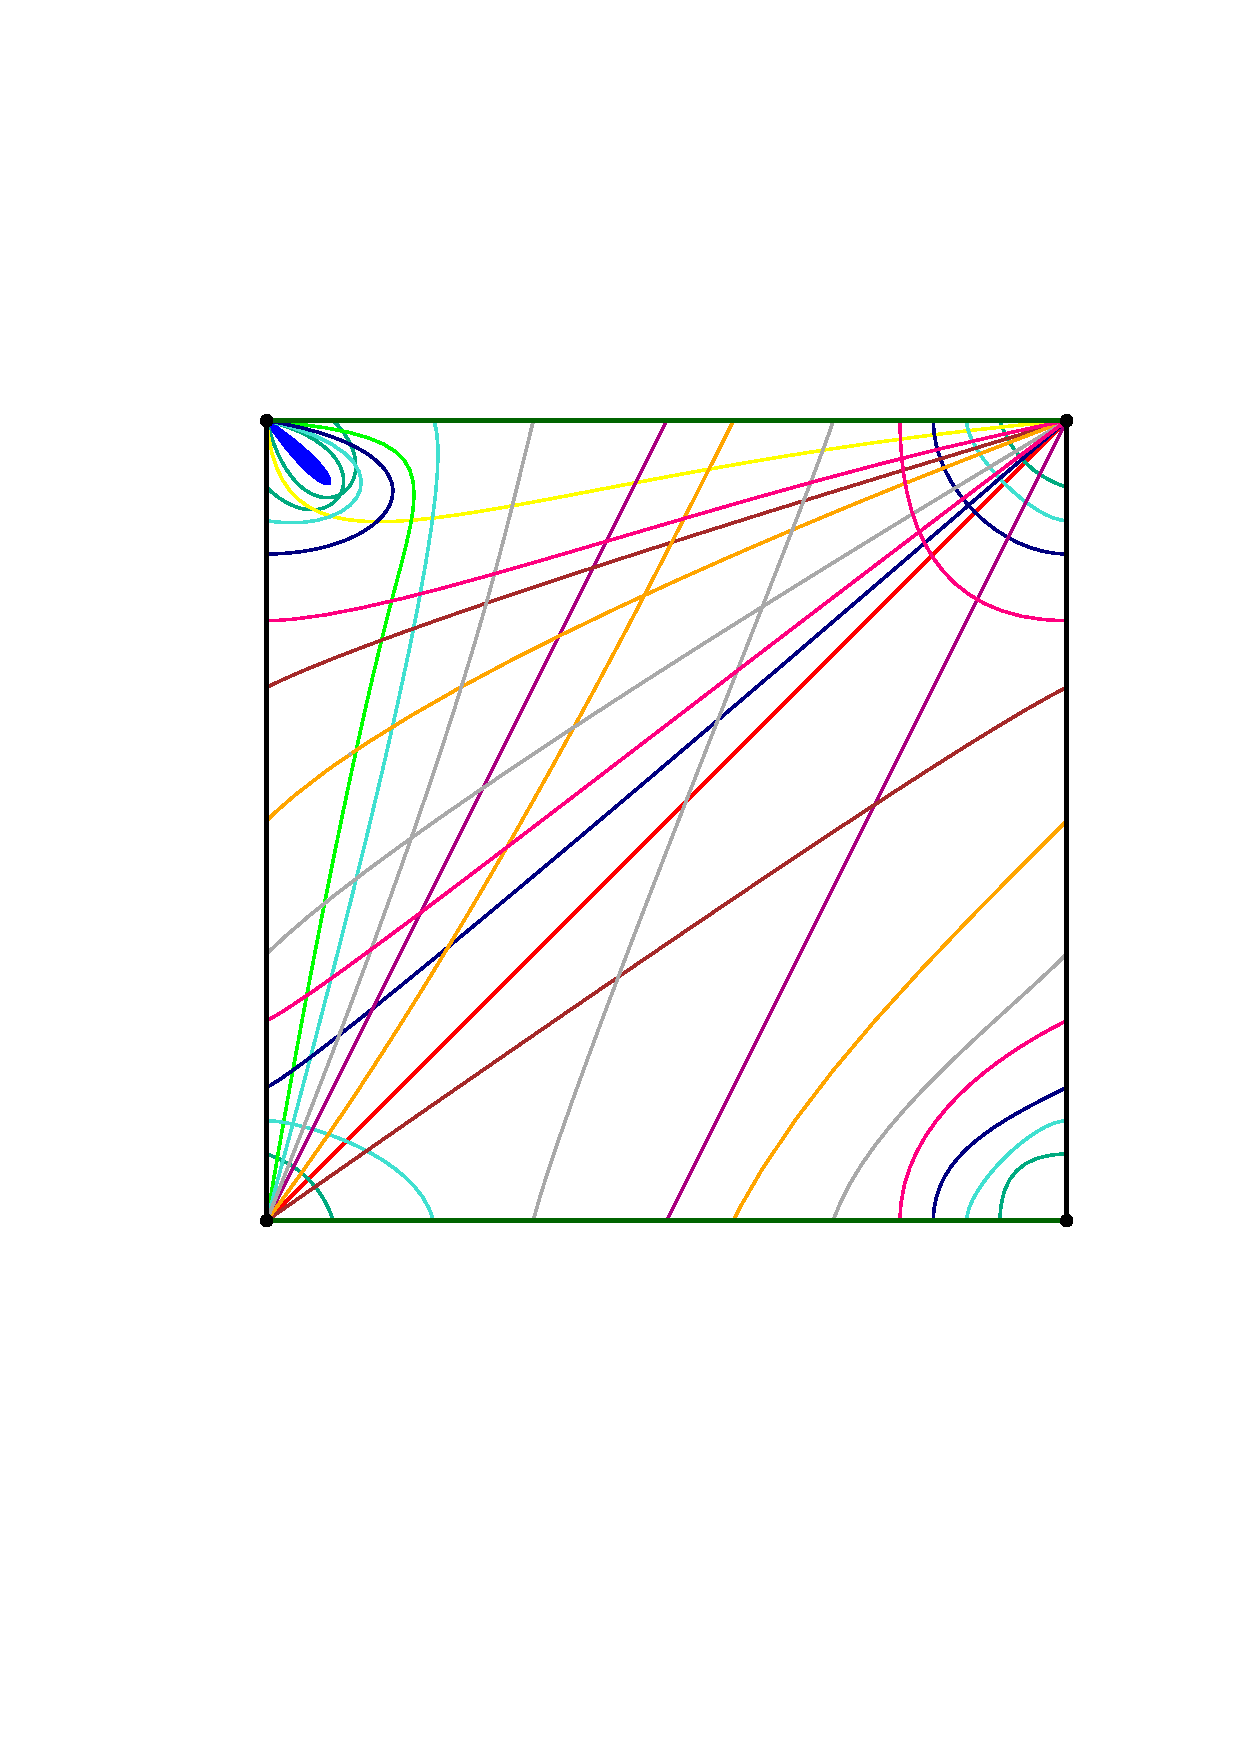
\includegraphics[scale=.42]{exTorusSquare}}
	\caption{A $2$-triangulation of a torus with a hole (in blue), whose universal cover is represented in \cref{fig:UCtorus}.}
	\label{fig:torus}
\end{figure}

\begin{theorem}
\label{generalFlip}
Any $k$-relevant edge of a $k$-triangulation on a surface can be flipped.
\end{theorem}

%%%%%%%%%%%%

\subsection{Examples}

An example of non-sequential flip

%%%%%%%%%%%%%%%%%%%%%%%%%%%%%%%%%%%%%%

\section{multitriangulations of the half-cylinder}

\begin{definition}
A \defn{half-cylinder} is a cylinder with no point on the upper border.
\end{definition}

\begin{figure}
\label{fig:saturatedHC2}
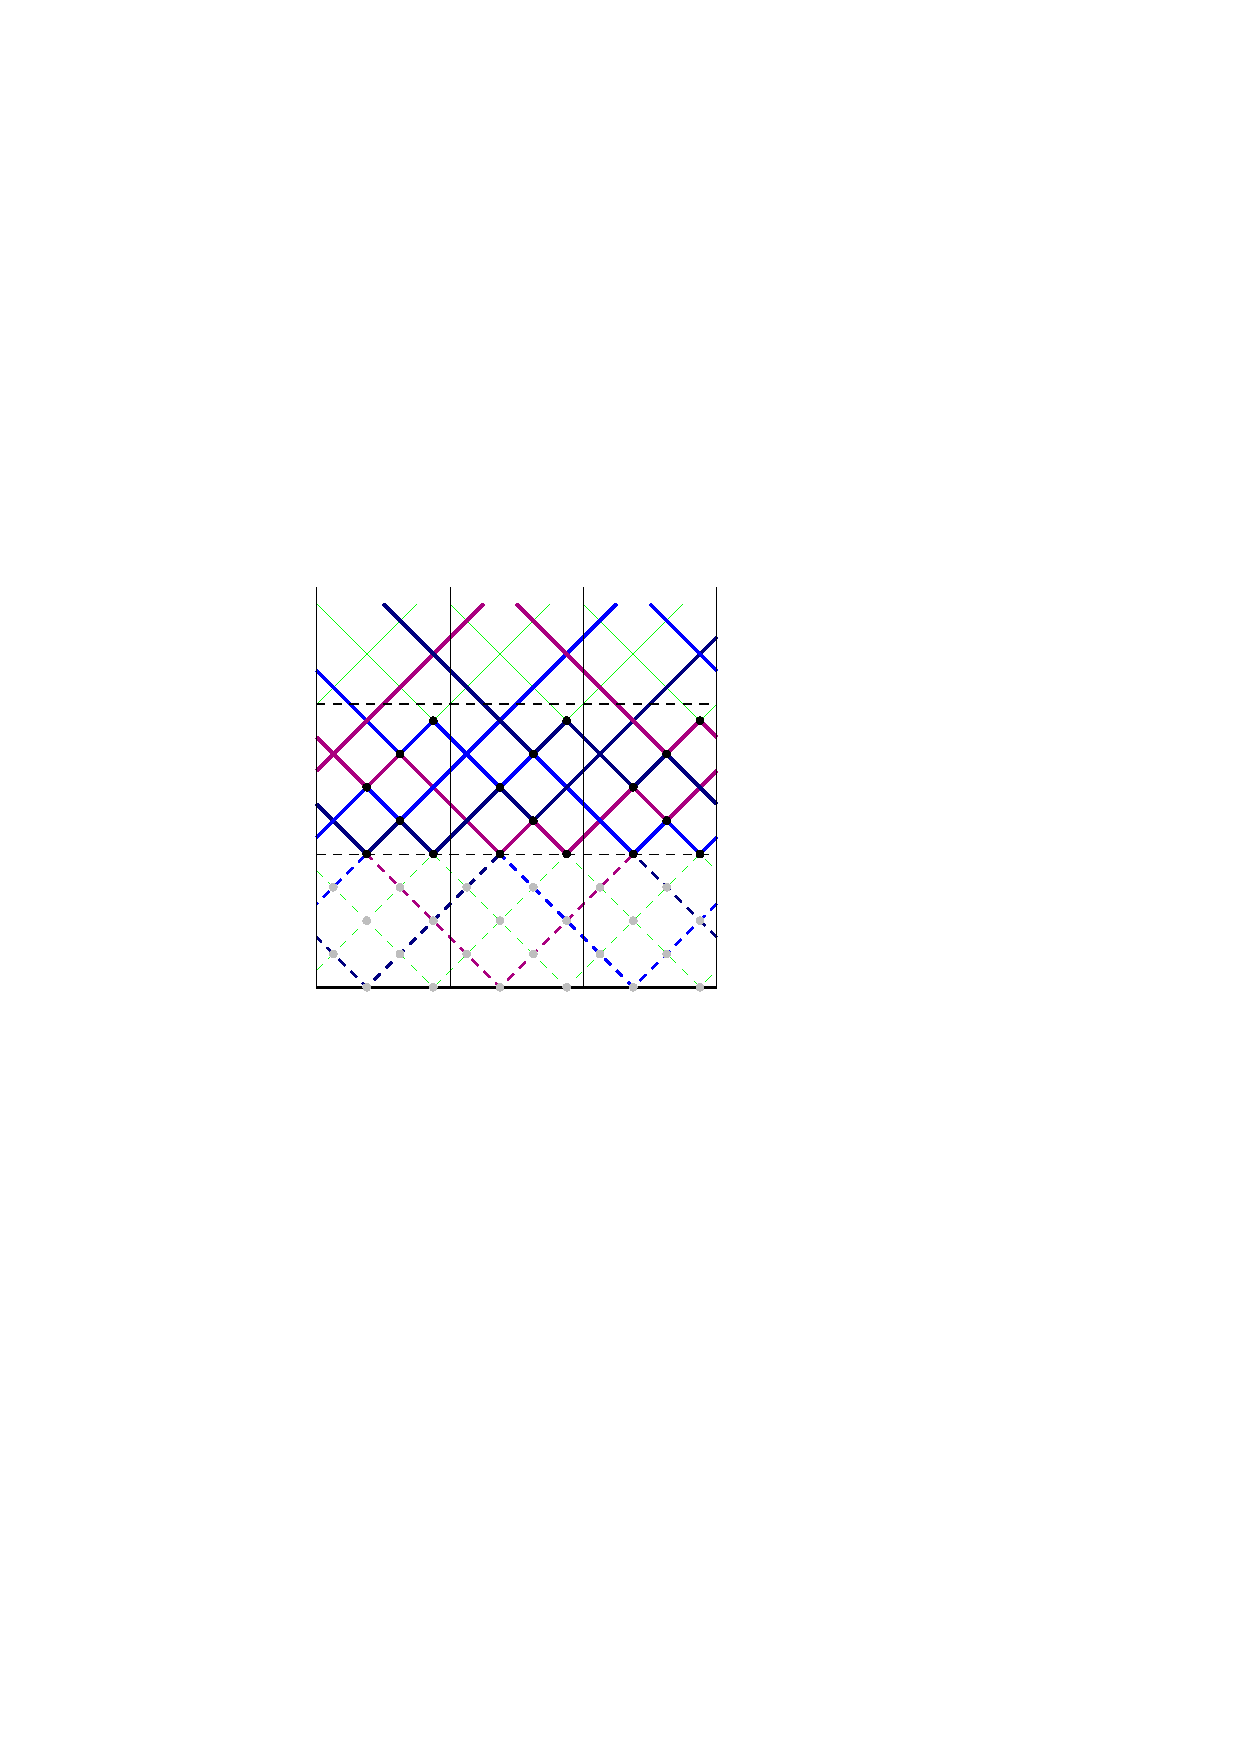
\includegraphics[scale=1]{saturatedHC}
\caption{representation...}
\end{figure}

%%%%%%%%%%%%

\subsection{Half-cylinder with $2$ marked points}

Consider the situation where the surface~$\surface$ is a cylinder with two points~$a,b$ on one boundary and none on the other.
The universal cover is an infinite band, with points~$a_{\ell}, b_{\ell}$ for~$\ell \in \Z$ alternating on one boundary (so that~$a_\ell+1 = b_\ell = a_{\ell+1}-1$).
For~$k \ge 1$ and a word~$w \eqdef w^1 \dots w^k \eqdef  \in \{a,b\}^k$, consider a set~$T_w$ of diagonals of~$\surface$ formed by
\begin{itemize}
\item the diagonals~$(w^i_\ell, w^i_{\ell}+k+i)$ for all~$i \in [k]$ and~$\ell \in \Z$,
\item all $k$-boundary and $k$-irrelevant diagonals~$(\epsilon_{\ell}, \epsilon_{\ell}+i)$ for~$i \in [k]$, $\epsilon \in \{a,b\}$ and~$\ell \in \Z$.
%\item the outer $k$-boundary diagonals~$(a_{\ell}, a_{\ell}+2k)$ for~$\ell \in \Z$.
\end{itemize}

\begin{figure}
	\capstart
	\includegraphics[page=2, scale=.5, clip, trim=15cm 0cm 17cm 0cm]{FNSk3p2} \\[.5cm]
	\includegraphics[page=3, scale=.5, clip, trim=15cm 0cm 17cm 0cm]{FNSk3p2}
	\caption{Two $3$-triangulations of a half cylinder related by a non-sequential flip. The edge~$a_ib_{i+2}$ is flipped to the edge~$b_ia_{i+3}$. These edges belong to two consecutive copies of the same $3$-star.}
	\label{fig:nonsequential}
\end{figure}

\begin{figure}
	\capstart
	\mbox{\includegraphics[page=6, scale=.5, clip, trim=21.2cm 0cm 24cm 6cm]{FNSk3p2} \quad \raisebox{1.7cm}{\includegraphics[page=4, scale=.5]{FNSk3p2}}} \\[.5cm]
	\mbox{\includegraphics[page=7, scale=.5, clip, trim=21.2cm 0cm 24cm 6cm]{FNSk3p2} \quad \raisebox{1.7cm}{\includegraphics[page=5, scale=.5]{FNSk3p2}}}
	\caption{The V (left) and H (right) representations of the $3$-triangulations of \cref{fig:nonsequential}.}
	\label{fig:nonsequentialVHrep}
\end{figure}

\begin{lemma}
\label{lem:noTwoDiagonalsEachLevel}
The sets
\begin{itemize}
\item $\set{(\epsilon_\ell, \epsilon_\ell+k+i)}{\epsilon \in \{a,b\} \text{ and } \ell \in \Z}$ for any~$i \in [k]$,
\item $\set{(\epsilon_\ell, \epsilon_\ell+k+i)}{\ell \in \Z}$ for any~$\epsilon \in \{a,b\}$ and~$i \ge k+1$,
\end{itemize}
all contain a $(k+1)$-crossing.
\end{lemma}

\begin{proposition}
For any~$k \ge 1$ and~$w \eqdef  \in \{a,b\}^k$, the set~$T_w$ is a $k$-triangulation of~$\surface$.
\end{proposition}

\begin{proof}
The maximality is immediate from \cref{lem:noTwoDiagonalsEachLevel}.
To see that~$T_w$ is $(k+1)$-crossing-free, we use the following strategy:
\begin{itemize}
\item the set of diagonals~$\set{(\epsilon_\ell, \epsilon_\ell+2k)}{\ell \in \Z}$ has no $(k+1)$-crossing for any~$\epsilon \in \{a,b\}$,
\item given any set~$X$ of pairwise crossing diagonals in~$T_w$, we can construct a new set~$X'$ of pairwise crossing diagonals in~$T_w$ by increasing the length of the smallest diagonal~$(u,v)$ of~$X$, provided this length is not~$2k$. Indeed, we just need to observe that the vertices~$u-1$ and~$v-1$ cannot be incident to diagonals of~$X$.
\qedhere
\end{itemize}
\end{proof}

\begin{corollary}
\label{coro:allkTriangCyclinder}
The set of $k$-triangulations of~$\surface$ is~$\set{T_w}{w \in \{a,b\}^k}$.
\end{corollary}

\begin{proof}
Any $(k+1)$-crossing free set of diagonals of~$\surface$ is a subset of a certain~$T_w$ by \cref{lem:noTwoDiagonalsEachLevel}.
\end{proof}

We denote by~$\delta_w^i$ the diagonal of~$\surface$ which lifts to the diagonals~$(w^i_\ell, w^i_{\ell}+k+1+i)$.

\begin{proposition}
%For any~$w \in \{a,b\}^k$ and~$i \in [k]$, the diagonal~$\delta_w^i$ of the $k$-triangulation~$T_w$ can be fli
For any~$w, w' \in \{a,b\}^k$ which only differ at position~$i \in [k]$, the $k$-triangulations~$T_w$ and~$T_w'$ are the only two $k$-triangulations~$\surface$ which contain~${T_w \ssm \{\delta_w^i\} = T_{w'} \ssm \{\delta_{w'}^i\}}$. In other words, any diagonal~$\delta_w^i$ in the $k$-triangulation~$T_w$ can be uniquely flipped.
\end{proposition}

\begin{proof}
By definition of~$T_w$ and~$T_{w'}$, we have~${T_w \ssm \{\delta_w^i\} = T_{w'} \ssm \{\delta_{w'}^i\}}$ so that the flip is possible.
It is unique by \cref{coro:allkTriangCyclinder}.
\end{proof}

\begin{remark}
The flip of $\delta_w^1$ is sequential (for the first flip, all points below $\delta_w^1$ are vertices of the star below~$\delta_w^1$ and we can determine which of these angles see each other; we have not worked out the other flips yet).
In contrast, the flip of~$\delta_w^i$ is not sequential for~$i \in \{2, \dots, k-1\}$ (since the common bisector is still of length~$k+1$).
\end{remark}

\begin{remark}
This is just an example of non-sequential flips on a cylinder. We need to understand all flips on a cylinder.
\end{remark}

%%%%%%%%%%%%

\subsection{Saturated multitriangulation of a half-cylinder}

\begin{definition}
Let $T$ be a \ktg of the half-cylinder with $p$ points. We denote $n_T^l$ the number of edges of length $l$ in $T$. We say that $T$ is \defn{saturated} if there exists $L>k$ such that:
\begin{itemize}
\item $n_T^l=p$, for any $l\leq k$ (these are $k$-irrelevant and $k$-boundary edges),
\item $n_T^l=p-1$ for $l\in[k+1,L-1]$,
\item $n_T^l=0$ for $l>L.$ 
\end{itemize}
\end{definition}

\begin{theorem}
\label{thm:flipSaturated}
Any $k$-relevant edges of a saturated multitriangulation of the half-cylinder can be flipped.
\end{theorem}

%%%%%%%%%%%%

\subsection{multitriangulations of the half-cylinder}

\begin{theorem}\label{thm:flipHalfCylinder}
Any edge of a $k$-triangulation of a half-cylinder can be flipped.
\end{theorem}

Let $\mathcal{C}_p$ be a cylinder with $p$ points $(v_i)_{i\in\mathbb{Z}/p\mathbb{Z}}$ on one border and no point on the other border. 
The successive copies of a point $v_i$ in $\overline{\mathcal{C}_p}$ are denoted $v_i^j$ for $j\in\mathbb{Z}$.

Let D be a $(k+1)$-crossing-free set of non-$k$-irrelevant diagonals of $\mathcal{C}_p$ containing (at least) the $k$-boundary diagonals of $\mathcal{C}_p$, and $d$ be a $k$-relevant diagonal of $D$. We denote $l_d$, $i_d$ and $j_d$ the length, and the index of the left and right extremities of $d$. Note that $l_d\geq k$ because $d$ is $k$-relevant, and $l_d\leq kp$ because $D$ is $(k+1)$-crossing-free. Note also that $i_d+l_d-j_d=0$ (in $\mathbb{Z}/p\mathbb{Z}$) by definition.

We represent $\mathcal{C}_p$ by a cylindric grid $G$ of width $p$ and height $kp-p+1$, where each column, indexed by $\mathbb{Z}/p\mathbb{Z}$, represent a point, and each row, indexed by $[k,kp]$ represent a diagonal length.
We represent each edge $d$ of $D$ by a symbol $\bullet$ at position $(i_d,l_d)$ in $G$.
We associate a directed lattice to the grid $G$, made of an edge going from any point $i,l$ to the point $i-1,l+1$, and an edge from any point $i,l+1$ to the point $i,l$, for $l<kp$ and $i\in\mathbb{Z}/p\mathbb{Z}$, as well as an edge going from point $i,kp$ to point $i,kp$ for any $i\in\mathbb{Z}/p\mathbb{Z}$.
We naturally call these edges the \emph{upper outgoing}, \emph{upper ingoing}, \emph{lower outgoing}, \emph{lower ingoing} edges of a point. Note that points of the form $i,k$ have no lower edges.

A face of $D$ is made of a succession of \emph{top} diagonals (that are above the face), and \emph{bottom} diagonals (that are below the face). Around a face, their can be $2$ successive bottom edges, but no $2$ successive top edges. An angle between two bottom diagonals is called \emph{upper angle}, an angle between a top and a bottom diagonals is called \emph{lower angle}.
The \emph{counterclockwise tour} of a face $f$ of $D$ is computed by the following procedure. Start from any diagonal $d$ of $f$, and perform the following operation until you get back to this original diagonal.
\begin{enumerate}
\item If $d$ is a top diagonal, set $d$ to be longest diagonal starting from $v_{i_d}$ and having length less than $l_d$. Note that this is well defined because $D$ contains the $k$-boundary diagonals, and a $k$-boundary diagonals cannot be a top diagonal.
\item Else, if $d$ is a bottom diagonal, and $l_d$ is the maximum length of an edge ending on point~$v_{j_d}$, then set $d$ to be the longest diagonal starting on point~$v_{i_d}$.
\item Else, set $d$ to be the shorted diagonal ending on point $v_{j_d}$ and having length more than~$l_d$.
\end{enumerate}
If this procedure does not terminates, it means that the corresponding face is not finite, but rather infinite and periodic.

This procedure can easily be performed graphically in the grid representation, by following the edges of the lattice. Step $1$ corresponds to following lower outgoing edges until meeting a $\bullet$; step $3$ corresponds to following upper outgoing edges until meeting a $\bullet$; and step $2$ corresponds to following upper outgoing edges until reaching height $kp$, and then following lower outgoing edges until meeting a $\bullet$.
In the grid representation, this procedure necessarily ends with a cycle $C_f$.

We call \emph{drift} the integer $\delta_f$ equal the total length of top diagonals of $C_f$ minus the total length of bottom diagonals of $C_f$.
Then $f$ is finite if and only if $\delta_f=0$.

\begin{conjecture}
$D$ is a $k$-triangulation if and only if it has $p-1$ faces, who all have drift $0$ and length $2k+1$.
\end{conjecture}

%%% brouillon = on

also, faces have $k$ top and $k+1$ bottom edges, in other words, only $1$ upper angle.

\begin{proof}[tentative proof]
If $D$ is a $k$-triangulation, then its faces have drift $0$ and length $2k+1$ because of \cref{thm:structureInfinite}.

We can give an example of a $k$-triangulations with $p-1$ $k$-stars. If we can prove that all $k$-triangulations of a surface have the same number of $k$-stars, then we proved the direct implication.

Now suppose $D$ has $p-1$ faces, who all have drift $0$ and length $2k+1$. 
If we can prove that all $k$-triangulations of a surface have the same number of $k$-stars, then $D$ is maximal. I can also give an enumerative argument for maximality, counting the number of $\bullet$ and empty spaces that we have to fill in the $p\times kp$ grid.

What's missing is to prove that $D$ has no $(k+1)$-crossing.
\end{proof}

%%% brouillon = off

Let $T$ be a $k$-triangulation of $\mathcal{C}_p$, $S$ a star of $T$, and $d$ a diagonal adjacent to $S$ on both sides.
Let $C_S$ be the cycle corresponding to $S$ in the grid representation.
Let $C_{S,d}^1$ be the subcycle of $C$ starting from the upper outgoing edge of $d$, and finishing at the lower ingoing edge of $d$.
Let $C_{S,d}^2$ be the subcycle of $C$ starting from the lower outgoing edge of $d$, and finishing at the upper ingoing edge of $d$.
The cycle $C$ is made of the succession of $C_{S,d}^1$ and $C_{S,d}^2$.

%%brouillon on
l'un est pair, l'autre impair et passe par l'infini. 
%%brouillon off

\begin{conjecture}
The cycles $C_{S,d}^1$ and $C_{S,d}^2$ have exactly $2$ intersection points.
\end{conjecture}

\begin{proof}[tentative proof]
The number of intersection points of two cycles on a cylinder is necessarily even. By definition, the $\bullet$ corresponding to $d$ is a point of intersection.

We need to prove that there cannot be more than $2$ intersection points.
\end{proof}

\begin{proof}[proof of \cref{thm:flipHalfCylinder}]
Let $T$ be a triangulation of $\mathcal{C}_p$, and $d$ a diagonal of $T$.
If $d$ is adjacent to two different stars, then it can be flipped in a sequential manner.

If $d$ is adjacent twice to the same star, then denote $d'$ the point of intersection between $C_{S,d}^1$ and $C_{S,d}^2$ which is not $d$.
Denote $C_{S,d}^{1,1}$ and $C_{S,d}^{1,2}$ the subpaths of $C_{S,d}^1$ going from $d$ to $d'$, and from $d'$ to $d$.
Denote $C_{S,d}^{2,1}$ and $C_{S,d}^{2,2}$ the subpaths of $C_{S,d}^2$ going from $d$ to $d'$, and from $d'$ to $d$.
The cycle $C$ is made of the cyclic concatenation of $C_{S,d}^{1,1}$, $C_{S,d}^{1,2}$, $C_{S,d}^{2,1}$, and $C_{S,d}^{2,2}$.

Now remove $d$ and add in $d'$. This creates a new face $S'$, corresponding in the grid representation to a cycle $C'$ made of the cyclic concatenation of $C_{S,d}^{1,1}$, $C_{S,d}^{2,2}$, $C_{S,d}^{2,1}$, and $C_{S,d}^{1,2}$.
Since $S'$ is made of the same paths as $S$, it as well has drift $0$ and length $2k+1$, so that what we obtain is a $k$-triangulation.
\end{proof}

%%%%%%%%%%%
%
%%%% rewrote begining above
%
%By consequence the walk can be entirely deduced from the disposition of the points. see \cref{fig:exLattice}.
%
%\begin{figure}\label{fig:exLattice}
%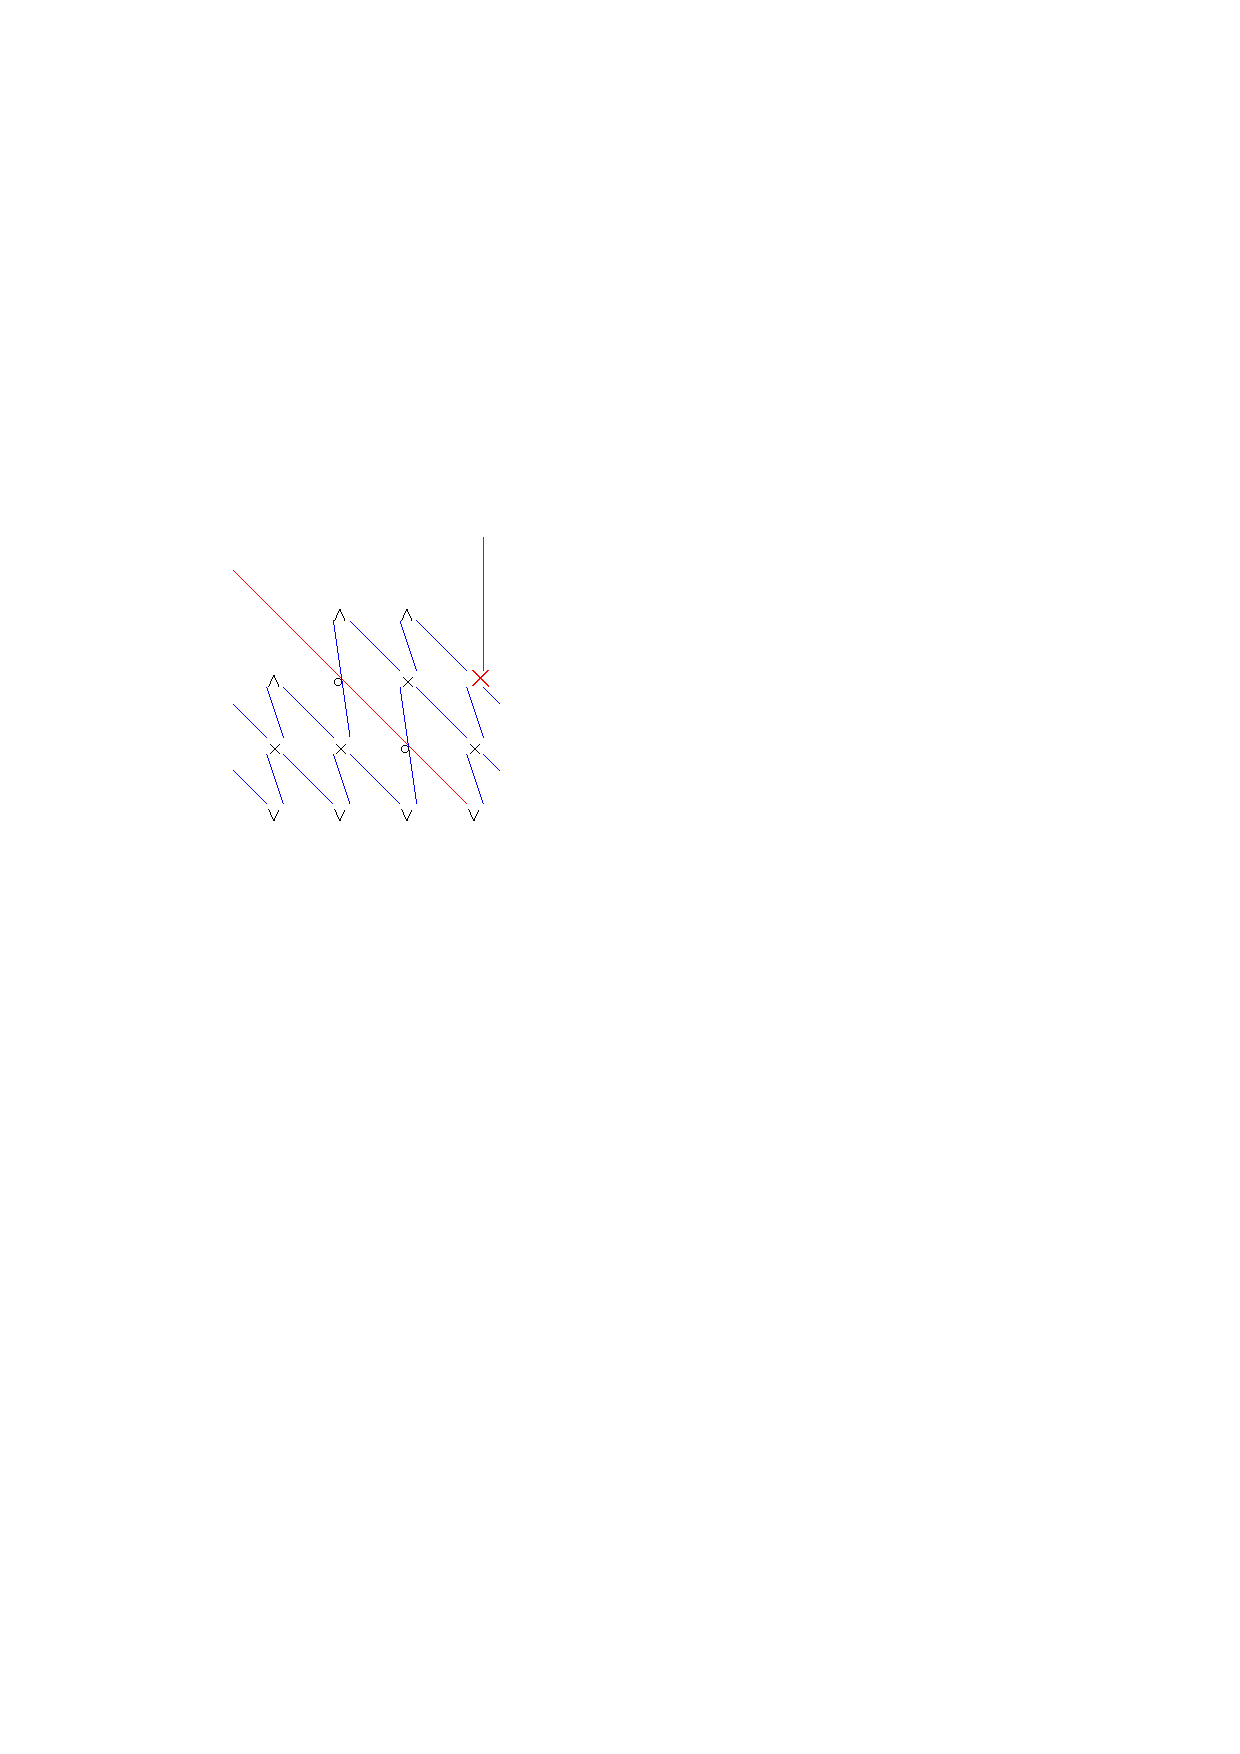
\includegraphics[scale=1]{latticeRepresentation}
%\caption{example of the lattice representation of $7$-triangulation with a unique star, on the half-cylinder with $4$ points.}
%\end{figure}
%
%%Since there is only one star, all $k$-border edges have to be part of the star. 
%We denote $l_{min}$ and $l_{\max}$ the minimal and maximal length of an edge of $S$.
%
%A $k$-star has $2k+1$ edges: $n_\vee+n_\wedge+2n_\times=2k+1$. It is on the upper side of $k+1$ of them and the lower side of $k$ of them: $n_\vee+n_\times=k+1$ and $n_\wedge+n_\times=k$.
%
%We group edges by successive pairs: an edge followed by a smaller edge. This corresponds in the lattice to a vertical descending edge, and in the cylinder to a left angle of the star. Only the red edge remain unmatched. When doing a tour of $S$, each pair makes you go to the left by a length corresponding to the height of the corresponding vertical edge, and the edge corresponding to the red point makes you go to the right by a length corresponding to the height of the red point. In the end of the tour, you have to get back to your initial position.
%
%By consequence, the total length of blue vertical edges, denoted $\diskelta$, has to be equal to the length of the edge corresponding to the red vertex, denoted $h$.
%
%NB (to be proved): an excursion in the lattice corresponds to a $k$-star if and only if it has length $k+1$ and exactly $1$ red point/edge, and $\diskelta=h$.
%
%
%Over any symbol $\vee$, there is a sequence of $\circ$ and $\times$, ended by a $\wedge$ or a red $\times$ (and potentially followed by another sequence). Inside each of these sequence,  we know that all vertical edges are visited by the excursion. By consequence: $\Delta=n_\wedge+n_\times+n_\circ$. 
%
%Let $l$ be a length such that $l_{min}<l<l_{max}$. Since the star is represented by a (connected) excursion, there exists a vertex $i$ such that $(i,l)$ has symbol $\circ$. By consequence, $n_\circ\geq l_{max}-l_{min}-1$.
%
%By unicity of the red $\times$, the symbol coming just after the red $\times$ has to have length strictly bigger. By consequence $h<l_{max}$.  Note also that $l_{min}\geq k$.
%
%By grouping everything together we obtain:
%
%\begin{align}
%0&=\diskelta-h \\
%&=n_\wedge+n_\times+n_\circ-h\\
%&=k+n_\circ-h\\
%&=(k-l_{min})+(l_{min}+n_\circ-l_{max}+1)+(l_{max}-1-h)
%\end{align}
%
%$k-l_{min}$ EST À L'ENVERS...  
%
%By consequence: $l_{min}=k$, $n_\circ=L-k-1$ and $h=L-1$.
%
%We showed that at each level between $k+1$ and $h$, there is exactly one point where the blue line goes through vertically. We can show in the exact same way that there is exactly one point where the blue line goes through diagonally.
%
%If we count the special edge, each star has exactly $1$ vertical edge and 1 diagonal edge at all level $l>k$.
%
%
%Note that we did not use the fact that the star is unique, so that this is true for any star of a triangulation of the half-cylinder. In particular, the number of star of such a triangulation is strictly smaller than $p$. see \cref{fig:2stars}.
%
%
%\begin{figure}\label{fig:2stars}
%\includegraphics[width=.98\linewidth,page=3]{latticeRepresentation}
%\caption{an example of a $2$-triangulation of the half cylinder with $2$ points and $2$ stars.}
%\end{figure}
%
%\medskip
%
%NOT TRUE ANYMORE, BECAUSE THEY ARE NOT $K$-TRIANGULATIONS (see ultrafat edges on picture) ET D'AILLEURS L_MAX>KP.
%However it may be that there are more than $k$ $\vee$. See \cref{fig:problem}. The first line should be the smallest such configuration. However it has no flippable edge, unlike the second one. In the second configuration, it is still easy to flip the unique flippable edge. As always, it suffices to exchange a blue crossing with a $\circ$ (as illustrated in the second row of \cref{fig:problem}). 
%DANS CES EXEMPLES ON A 	$l_{max}>kp$...
%
%\begin{figure}\label{fig:problem}
%\includegraphics[width=.98\linewidth,page=2]{latticeRepresentation}
%\caption{problems may occur...}
%\end{figure}

%%%%%%%%%%%%

\subsection{Non-sequential flips and restriction to the cylinder}

Consider a $k$-triangulation~$T$ of a surface~$\surface$.
Let~$\bar T$ be the corresponding infinite $k$-triangulation of the universal cover~$\bar \surface$.
We want to show that any $k$-relevant arc~$\alpha$ of~$T$ is flippable.
The natural idea is to flip sequentially all copies~$\bar\alpha$ of the arc~$\alpha$ in~$\bar T$.
However, this only works if, at any point of this procedure, the flip of any copy~$\bar\alpha$ in~$\bar T$ does not modify the flip of the other copies of~$\alpha$ in~$\bar T$.
We say that the flip of~$\alpha$ in~$T$ is \defn{sequential} when this procedure works, and \defn{non-sequential} otherwise.

\begin{example}
A non sequential flip.
\end{example}


The goal of this section is to show that non-sequential flips in $k$-triangulations of any surface~$\surface$ just boil down to non-sequential flips of $k$-triangulations of a cylinder~$\cylinder$.
For this, consider an arc~$\alpha$ of a $k$-triangulation~$T$ of~$\surface$, and let~$S,S'$ be the two $k$-stars of~$T$ containing~$\alpha$.
We distinguish three cases:\mathias{3?}
\begin{itemize}
\item If~$S$ and~$S'$ are distinct $k$-stars of~$T$, then $\alpha$ appears only once in~$S$ and in~$S'$. Consider a copy~$\bar\alpha$ of~$\alpha$ in~$\bar T$ and the copy~$\bar S$ (resp.~$\bar S'$) of~$S$ (resp.~$S'$) in~$\bar T$ containing~$\bar\alpha$. Remember from \cref{sec:infiniteMultitriangulations} that the flip of~$\bar\alpha$ in~$\bar T$ only depends on and only modifies the two $k$-stars~$\bar S$ and~$\bar S'$. Since~$\bar\alpha$ is not contained in any other copy of~$S$ and~$S'$ in~$\bar T$, the flip of~$\bar\alpha$ in~$\bar T$ does not modify the flip of the other copies of~$\alpha$ in~$\bar T$. Therefore the flip is sequential.
\item Assume now that~$S = S'$ so that~$\alpha$ appears twice in~$S$. Let~$\bar\alpha$ and~$\bar\alpha'$ be two copies of~$\alpha$ in a copy~$\bar S$ of~$S$ in~$\bar T$. Let~$\pi$ be the homomorphism of~$\bar\surface$ such that~$\pi(\bar\alpha) = \bar\alpha'$. We consider the collection~$\bar U$ of arcs of stars~$\pi^i(\bar S)$ for~$i \in \Z$. Perform all identifications of two consecutive vertices of~$\bar U$ that do not uncross any pairs of arcs of~$\bar U$. These identifications can be performed in any order. The result~$\bar V$ is a $k$-triangulation of an infinite polygon whose homomorphism group is generated by~$\pi$. Therefore, $\bar V$ is a covering of a $k$-triangulation~$V$ of a cylinder~$\cylinder$.
\end{itemize}

\begin{theorem}
\label{thm:decompCylinder}
The surface obtained this way is a half-cylinder.
\end{theorem}

Combined with \cref{thm:flipSaturated,thm:uniStarSaturated}, we obtain \cref{generalFlip}.


Existe-t-il des mutlitriangulations avec plusieurs étoiles, dont une qui touche sa copie +1, et qui touhce tous les points.



\bibliographystyle{alpha}
\bibliography{multiTrig}

\end{document}
